\documentclass{llncs}
%
\usepackage{graphicx}
\usepackage{placeins}
%\usepackage{hyperref}

\usepackage{comment}
\usepackage{needspace}
\usepackage{url}
\usepackage{xcolor}
\usepackage{color}
\usepackage[ruled]{algorithm2e}

% correct bad hyphenation here
\usepackage{makeidx}  % allows for indexgeneration
\usepackage{fancyvrb}
\usepackage{amsmath, amssymb}
\usepackage{epsfig}
\usepackage{setspace}
\usepackage{multirow}
\usepackage{subfigure}
\usepackage{verbatim}
\usepackage{listings}
\usepackage{wrapfig}
%\usepackage{hyperref}
%\usepackage{xltxtra}
\newcommand{\REM}[1]{}
\usepackage{color}
\newcommand {\TODO}[1]{\textcolor{red}{TODO #1}}

\newcommand{\othertm}{\textsuperscript{$\star$}}
\newcommand{\regtm}{\textsuperscript{\textregistered{}}}
\newcommand{\tm}{{\scriptsize\texttrademark{}}}

%\newcommand{\descheader}[1]{{\needspace{3\baselineskip}\vspace{1em}\noindent \fbox{#1}}}


%
%\setlength{\textfloatsep}{0.4cm} 
\begin{document}
%
\mainmatter              % start of the contributions
%
%\title{A Proposal from OpenMP to Address Interoperability Challenges for Parallel Programming} %
\title{A Proposal to OpenMP for Addressing the CPU Oversubscription Challenge}
%Interoperability Challenges of Parallel Programming} %
%\title{A Portable Abstraction for Task Parallelism and Data Movement in Hierarchical Multiprocessors} %
%\titlerunning{Hamiltonian Mechanics}  % abbreviated title (for running head)
%                                     also used for the TOC unless
%                                     \toctitle is used
%
\author{
	Yonghong Yan\inst{1}$^{,}$\inst{5} \and
	Jeff R. Hammond\inst{2}$^{,}$\inst{5} \and
%	Ali Alqazzaz\inst{1} \and
	Chunhua Liao\inst{3} \and
	Alexandre E. Eichenberger\inst{4}$^{,}$\inst{5} 
}

\institute{
    Department of Computer Science and Engineering, Oakland University, 
    \email{yan@oakland.edu}
    \and
    Parallel Computing Lab, Intel Corp.,
    \email{jeff\_hammond@acm.org}
    \and
    Center for Applied Scientific Computing, Lawrence Livermore National Laboratory,
    \email{liao6@llnl.gov}
    \and
    Thomas J. Watson Research Center, IBM, 
    \email{alexe@us.ibm.com}
    \and
    OpenMP Interoperability Language Subcommittee
}
\maketitle              % typeset the title of the contribution

\begin{abstract}
OpenMP has become a very successful user-model for developing parallel applications. 
However, there are still some challenges in terms of OpenMP interoperability. 
In this paper, we introduce some extientions to the OpenMP runtime library realted to the interoperability problem. 
Also, we evaluate and compare the performance of the different waiting thread behaviours (PASSIVE \textbar ACTIVE). 
In addition, we introduce a new function to shutdown or unload the whole runtime library when exiting the parallel 
region to prove that It would take longer time than awakening a sleeping thread.
\end{abstract}
%

%\keywords
%Java, GPU, High Performance 
\section{Introduction}
\label{sec:intro}
%High-performance computing (HPC) applications must exploit parallelism
%in order to take advantage of all of the hardware resources of
%modern multicore nodes, potentially with some form of heterogeneity
%(e.g. specialized coprocessors).
%Obviously, there are a number of ways to map algorithmic concurrency
%to hardware parallelism, which on general purpose processors rely
%upon either multi-threading or multiprocessing, which are different
%from the user perspective but very similar from the perspective of
%the operating system and hardware.

OpenMP is the most popular programming model for multi-threading in HPC,
although it is far from the only one.
Other portable threading models that may be used in HPC include
POSIX threads,
Intel\regtm{} Threading Building Blocks (TBB)~\cite{pheatt2008intel},
%\footnote{TBB is build on top
%of POSIX threads (at least on Linux systems), and is portable to
%processors from AMD, ARM, IBM, Intel and other vendors.},
ISO C11 and C++ threads, Cilkplus and
OpenCL, to name a few. 
In addition to the explicit use of threads in HPC applications,
threads may be used implicitly in language concurrent features such as
ISO C++11 {\sf std::async} and {\sf std::future},
ISO Fortran 2008 {\sf DO CONCURRENT} and coarray images.
%\footnote{
%The Fortran standard does not specify how coarray images are implemented,
%but it almost certainly involves either OS threads or OS processes.}.
Both compute and communication libraries may use threads;
compute libraries that implement BLAS, LAPACK or FFT functions
currently use at least four different threading models internally and
communication libraries such as MPI may spawn threads to implement asynchronous progress.
%Finally, in addition to multiple forms of threads, there may be multiple
%processes executing the application code on the node, the most obvious example
%of which is when MPI is used.  However, for purposes of this paper, we will
%not consider multiprocessing differently from multi-threading,
%due to their similarities as it pertains to interoperability problems.

Large-scale parallel applications are typically developed using multiple parallel programming APIs 
aforementioned, e.g. the hybrid MPI+OpenMP, and using one or multiple pre-built parallel scientific
libraries such as Intel Math Kernel Library (MKL)~\cite{wang2014intel}.
Each of these APIs often has its own runtime system to handle scheduling of work units 
and management of computational and data movement tasks. 
One of the challenges for using multiple models in one application is the interoperability and
interaction of their threading runtime, for example the issues of naming conflicts and resource
oversubscription. 

%. Composability are closely related, while the interoperability sounds to improve the interactions between multiple models
%while composability is meant to improve the modular use of OpenMP with itself and other models. One is from the aspect of system while 
%the other is more concerned with software engineering. Both should be considered when developing solutions. 

This paper reports our proposal to OpenMP for combating the resource oversubscription challenge as efforts from
the OpenMP Interoperability language subcommittee. The work makes three contributions: 1) a study 
of interoperability challenge in OpenMP and other parallel APIs and the limitation 
of the current standard to address this challenge; 2) proposed extensions to OpenMP to improve the thread
management to enhance OpenMP to interoperate with other threading models; 3) evaluation and performance
study that demonstrate the effectiveness of the proposed solution and provide guideline for selecting thread
waiting policies according to the oversubscription ratios. 
%Though proposed as OpenMP extensions, the solution 
%and approach are applicable to other threading libraries and parallel programming languages. 
We think the similar challenge exists in other threading based libraries and language implementations, and believe
the solutions we provided  will work for them too.  

%\begin{comment} % the paragraph above already introduces layout of the paper
The rest of the paper is organized as follows: Section~\ref{sec:challenges} discusses the interoperability 
use cases, challenges and motivations. 
 Section~\ref{sec:proposal} describes the proposed solutions for OpenMP. % runtime routines.
 Section~\ref{sec:implementation} presents our implementation and evaluation. 
 Finally, Section~\ref{sec:related} discusses related
work and Section~\ref{sec:conclusion} contains our conclusions.
%\end{comment}






%With those identified classes and use cases, we studied the performance impacts of multiple parallel runtime that 
%do not interoperate well with either including oversubscription and memory affinity confliction. We then propose language 
%extensions to OpenMP to address the interoperability challenges of parallel programming. 
\begin{comment}

Applications are using multiple threading models.
Common ones include OpenMP, POSIX threads, TBB, OpenCL.
Now that ISO C11 and C++11 both have threads, and C++11 has
std::async, std::future, etc., programmers have many
ways to create threads in a program.

Libraries are written independent of applications, will use what is best
aligned with their design, or which is most interoperable (like OS threads).
Some libraries may need to be called from threaded region, but often not.

Runtimes often use threads, but in a very different way from applications.
Example of MPI or PGAS runtime with communication helper threads.
OpenMP task cannot be used here since cannot use outside of parallel region.
Runtime threads must interact with OS in deep way, so OS threads make sense.

Primary problem is oversubscription of hardware threads, which causes
major performance issues, particularly on HPC-oriented lightweight operating systems
(e.g. IBM Blue Gene CNK).

Secondary problem of affinity.
Even if software threads do not oversubscribe hardware threads,
are software threads running on the right set of resources at the right time.
Best performance often achieved with affinity binding to specific resources,
which creates oversubscription for a specific resource, even if not globally.

Three approaches:
(1) explicit thread creation
(2) wait policy
(3) quiesce

(1) assumes every client of threads buys into it, which is not going to happen,
even though the API is aligned with POSIX/Windows/Solaris thread APIs.
Example of clone() for Cray XT Seastar/Portals3 in ARMCI.
However, may be particularly useful for HPC systems, where full-blown POSIX
threads are too much, and simple OS threading model is sufficient
(IBM Blue Gene is a good example of this).
MPI libraries support POSIX/Solaris/Windows threads already -- would
not be difficult to support OpenMP abstraction for OS threads,
at least in HPC environments.

(2) wait policy causes threads to back off and potentially go to
sleep while other threads are running.
However, these sleeping threads are parked in the kernel and may
still cause some OS scheduling overhead, if not sufficiently passive.
How long before threads back off completely?
Will this always happen before other threading model is running?
Do sleeping threads have affinity consequences?  If pinned, possibly.
Even Intel monitor-mwait consumes the hardware thread
(Blue Gene interrupt/wakeup unit does not).
Aggressive wait policy is great for interop but hurts latency.
Have to pull all threads out of sleep for new parallel region.
Forces application to pay tax on every fork-join when not required.
Some OpenMP codes do lots of fork-join, and it is likely optimal to
spin-wait in serial regions, at least for a short period, to ensure
the lowest latency of parallel region creation.

(3) is heavy hammer but allows for bulk sync phased interop, which
is especially useful for libraries.
Likely more expensive than most aggressive wait policy, but the cost
of recreation is only paid after when quiesce is used explicitly, when needed.
In some cases, quiesce may just invoke deep sleep, not actually destroy
thread pool, but this still permits the threads to use low-latency
wait policy between join and fork.

\end{comment}

\begin{comment}
Large-scale parallel applications are typically developed using multiple parallel programming models in 
a hybrid fashion, e.g. MPI+OpenMP, and using one or multiple pre-built scientific and/or platform-specific libraries such as Intel Math Kernel Library (MKL)~\cite{wang2014intel}.
Each of these programming models and libraries often has its own runtime library to handle scheduling of work units and management of computational
and data movement tasks. 
There have been challenging issues for using these models in one application, including 
compatibility issues for compiling and linking, oversubscription of resources at runtime, and the naming conflicts that 
programmers have to create workaround wrappers to deal with.

This paper proposes solutions to the interoperability and composability challenge faced by the OpenMP programming interface, including those
between multiple OpenMP implementations and/or multiple OpenMP runtime instances of the same implementation, OpenMP 
with native threads (PThreads and Windows Native threads), OpenMP with other threading languages and libraries such 
as C++11, TBB and Cilkplus, and OpenMP with inter-node programming models such as MPI and PGAS. 
We think the similar challenges exist in other threading based libraries and language implementations;
the solutions we provide here may work for them too.
%, and believe the solutions we provided  will work for them too.  

Interoperability and composability are closely related, while the interoperability sounds to improve the interactions between multiple models
while composability is meant to improve the modular use of OpenMP with itself and other models. One is from the aspect of system while 
the other is more concerned with software engineering. Both should be considered when developing solutions. 

For parallel programming languages and libraries, most implementations rely on system native threading (PThreads or Windows Native threads) 
mechanisms to acquires system resources. Each implementation of the same or different programming models has their own mechanism for scheduling
user-level tasks and operations, which is the core part of a runtime system. 
The interoperability challenges are then concerned with how much we want two or more 
runtime instances (for the same or different high-level programming interfaces) to interact with other other for computational resource sharing
and data movement. Thus solutions to these challenges are more in the scope of runtime implementation, than in the level of programming
interfaces and compiler transformations. 
\TODO{I guess there might be language features enabling interoperability. Also are runtime library interfaces part of programming interfaces??}

\end{comment}

\REM{
\subsection{What is an OpenMP?}
OpenMP is an implementation model to support the implementation of parallel algorithms. It is primarily designed for shared memory multiprocessors. The goal of OpenMP is to provide a standard and portable API for writing shared memory parallel programs~\cite{dagum1998openmp}. 

OpenMP takes a directive-based approach for supporting parallelism. It consists of a set of directives that may be embedded within a program written in a base language such as Fortran, C, or C++. There are two compelling benefits of a directive-based approach that led to this choice: The first is that this approach allows the same code base to be used for development on both single-processor and multiprocessor platforms; on the former, the directives are simply treated as comments and ignored by the language translator, leading to correct serial execution. The second related benefit is that it allows an incremental approach to parallelism—starting from a sequential program, the programmer can embellish the same existing program with directives that express parallel execution. These directives may be offered within any base language (within the C/C++ languages, directives are referred to as “pragmas”). In addition to directives, OpenMP also includes a small set of runtime library routines and environment variables. These are typically used to examine and modify the execution parameters. The language extensions in OpenMP fall into one of three categories: control structures for expressing parallelism, data environment constructs for communicating between threads, and synchronization constructs for coordinating the execution of multiple threads~\cite{chandra2001parallel}.
\subsection{How does OpenMP work?}
OpenMP uses a fork/join execution model. OpenMP provides two kinds of constructs for controlling parallelism. First, it provides a directive to create multiple threads of execution that execute concurrently with each other. The only instance of this is the parallel directive. Second, OpenMP provides constructs to divide work among an existing set of parallel threads. An instance of this is the do directive. 

An OpenMP program always begins with a single thread of control that has associated with it an execution context or data environment. This initial thread of control is referred to as the master thread. When the master thread encounters a parallel construct, new threads of execution are created along with an execution context for each thread. Each thread has its own stack within its execution context. The execution context for a thread is the data address space containing all the variables specified in the program. Multiple OpenMP threads communicate with each other through ordinary reads and writes to shared variables.
\subsection{OpenMP Runtime Library}
The OpenMP API runtime library routines are external procedures. The return values of these routines are of default kind, unless otherwise specified. Runtime library provides interface to the compiler. The runtime interface is based on the idea that the compiler ``outlines`` code that is to run in parallel into separate functions that can then be invoked in multiple threads. OpenMP provides several runtime library routines to assist you in managing your program in parallel mode. Many of these runtime library routines have corresponding environment variables that can be set as defaults. The runtime library routines enable you to dynamically change these factors to assist in controlling your program. In all cases, a call to a runtime library routine overrides any corresponding environment variable. 

Generally, we can analyze the architecture into two perspectives: the parallelization regions and the data.
\begin{enumerate}
	\item Region perspective.
	We use “parallel” to automatically create multi-threads. And each thread will be executed without order. However, we can use ordered clause to guarantee the code be executed in sequence. There are different types of parallel regions:
	\begin{itemize}
		\item Section means the task is assigned to each thread.
		\item Single means the task is assigned to a random thread.
		\item Master means the task is executed in the master thread.
	\end{itemize}
	For the default parallel regions, we can use “schedule” to design a way to assign tasks to different threads. Generally, we can implement this assignment in three ways:
	\begin{itemize}
		\item Static: equally assign them to n threads.
		\item Dynamic: assign them to the idle thread only.
		\item Guided: implement the dynamic assignment reductively.
	\end{itemize}
	\item Data perspective.
	We have two kinds of variables. Variables that are defined before parallel region are shared among every thread, while those defined in parallel regions can be only accessed by certain threads. We use “threadprivate” to change those shared variables into a private one for each thread. This is done by generating a new private variable for every single thread. For those shared variables, we must pay attention to the data race problem, which defined as two different memory operations are trying to use a same variable, and different execution order may lead to different results. To solve this problem, we can use “critical” or “atomic” directive to guarantee that the data can be only accessed by one thread at a time. We can also set “barriers” to make sure all threads have been executed before starting any new threads. Sometimes the update of certain variables are stored only in registers, we can use “flush” to directly write the data back to memory to make sure that other threads will use the data that already been updated.
\end{enumerate}
}


\section{Use Cases and Challenges of Interoperability}
\label{sec:challenges}
%\TODO{Introduction mentions interoperability between two OpenMP runtimes. But this section does not mention this. That is part of use case #2}

\subsection{Use Cases of OpenMP Interoperability}
We have identified four use cases of OpenMP interoperating with itself and other parallel programming models. 
\subsubsection{Interacting With User threads}
\textbf{Definition}
A user thread is a thread that is not created by OpenMP implementation. A user thread 
could become an OpenMP initial thread. 

The most common example of user threads are POSIX Threads, 
usually referred to as Pthreads with implementation available on most Unix-like 
POSIX-compliant systems. There are also implementations of other thread libraries, 
for example, Windows Native threads and language based threading support such as 
Java threads or others (e.g. qthreads). 

Figure~\ref{fig:pthread-omp} shows an example of having three user 
threads (two PThreads and one thread of the main program) in an OpenMP program. 
The two three threads execute in parallel after the two PThreads are created. 
Each thread calls a function that will enter into
OpenMP threading parallelism. So they all become OpenMP initial threads. How the 
user threads (PThreads in this example) interact with the OpenMP threading mechanisms
in the runtime is up to the implementation. They may share the same OpenMP runtime
instance or each has its own OpenMP runtime instance. 

\begin{figure}[t]
\centering
  \fbox{
 % \lstset{basicstyle=\ttfamily\scriptsize,language=c}
  \lstset{basicstyle=\ttfamily\scriptsize,language=c,numbers=left, %,frame=single,
  deletekeywords={int,if,else,while},
  morekeywords={pragma,omp,target,device,map,
  tofrom,to,from,alloc,parallel,shared,reduction,data,collapse,
  private,dist_iteration,match_range,halo,exchange},
  numbersep=12pt,numberstyle=\color{red}}
  \lstinputlisting{pthread-omp.c}

}
\caption{Three user threads (two Pthreads and one main thread) with OpenMP}
  \label{fig:pthread-omp}
\end{figure}

\subsection{Impacts and Discussions}
A user thread in a program adds additional level(s) in the overall ``threading''
hierarchy of a program. Those additional levels could be on top of OpenMP threading 
mechanism when a user thread becomes an OpenMP initial thread that creates OpenMP thread
parallelism, or beneath the OpenMP threading mechanism when an OpenMP thread spawns 
a user thread, or the the mix of both. In the example from Figure~\ref{fig:pthread-omp}, 
one can view this in a two-level threading parallelism: the top level user thread 
parallelism and the bottom level OpenMP threading parallelism.

These additional levels of threading increase the complexity of a program, both for 
users in the aspect of reasoning the parallel and synchronization behavior of a program, 
and also for the implementation and runtime system in terms of resource management and 
interactions. Adding to the complexity is the facts that a user thread may be created 
through a call to a library function whose paralelism (OpenMP) behavior is not known to 
the callee. Typical issues for example: 
\begin{itemize}
\item Does each user thread use the same OpenMP runtime libraries or not? 
	If not using the same library, how to handle symbol name 
	conflicts of two more different OpenMP runtime libraries. 
\item For user threads that use the same OpenMP runtime library, does the user threads each create its own runtime instance or they share one?
\item For user threads each of which has its own runtime instance (from the same or 
	different runtime library), how to coordinate the resource management among those
	runtime instances to address such issues as oversubscriptions and the affinity
	between user threads?
\end{itemize}

It is important to note that approaches to address those issues are very implementation
dependent, requiring protocol and agreement in the runtime behavior and/or interfaces 
of different OpenMP implementations. It may not be realistic to solve some of the issue
from the language standard, and should be left to users to deal with them. In this
aspect, we still hope this report could provide userful information and practices 
for users. 



\subsubsection{Interacting with Other OpenMP Programs}
Often a parallel machine is shared by users running multiple programs at the same time.
It is very likly that multiple OpenMP programs coexist within the same computation node. 
The OpenMP programs can be compiled by a same OpenMP compiler or different compilers. 
Current, an OpenMP implementation, including its runtime, assumes that it fully occupies the entire computation node,
without considering the possibility of existence of other running OpenMP programs and their supportive OpenMP runtime instances. 
The coexistence of multiple OpenMP runtime instances raises the following questions:
\begin{itemize}
\item How many OpenMP programs are running currently?
\item Which OpenMP runtime system is being used by a running OpenMP program?
\item What resources are used by each of them?
\item How do the concurrently executing OpenMP programs interact with each others to ensure optimal resource utilization?
\end{itemize}


\subsubsection{Interacting With Other Parallel Systems or Libraries}
It is now very common that an application uses multiple parallel libraries at the same time, which could be developed 
using OpenMP, TBB, Cilkplus, C++11, and other parallel libraries. 

\begin{figure}[h!]
  \centering
      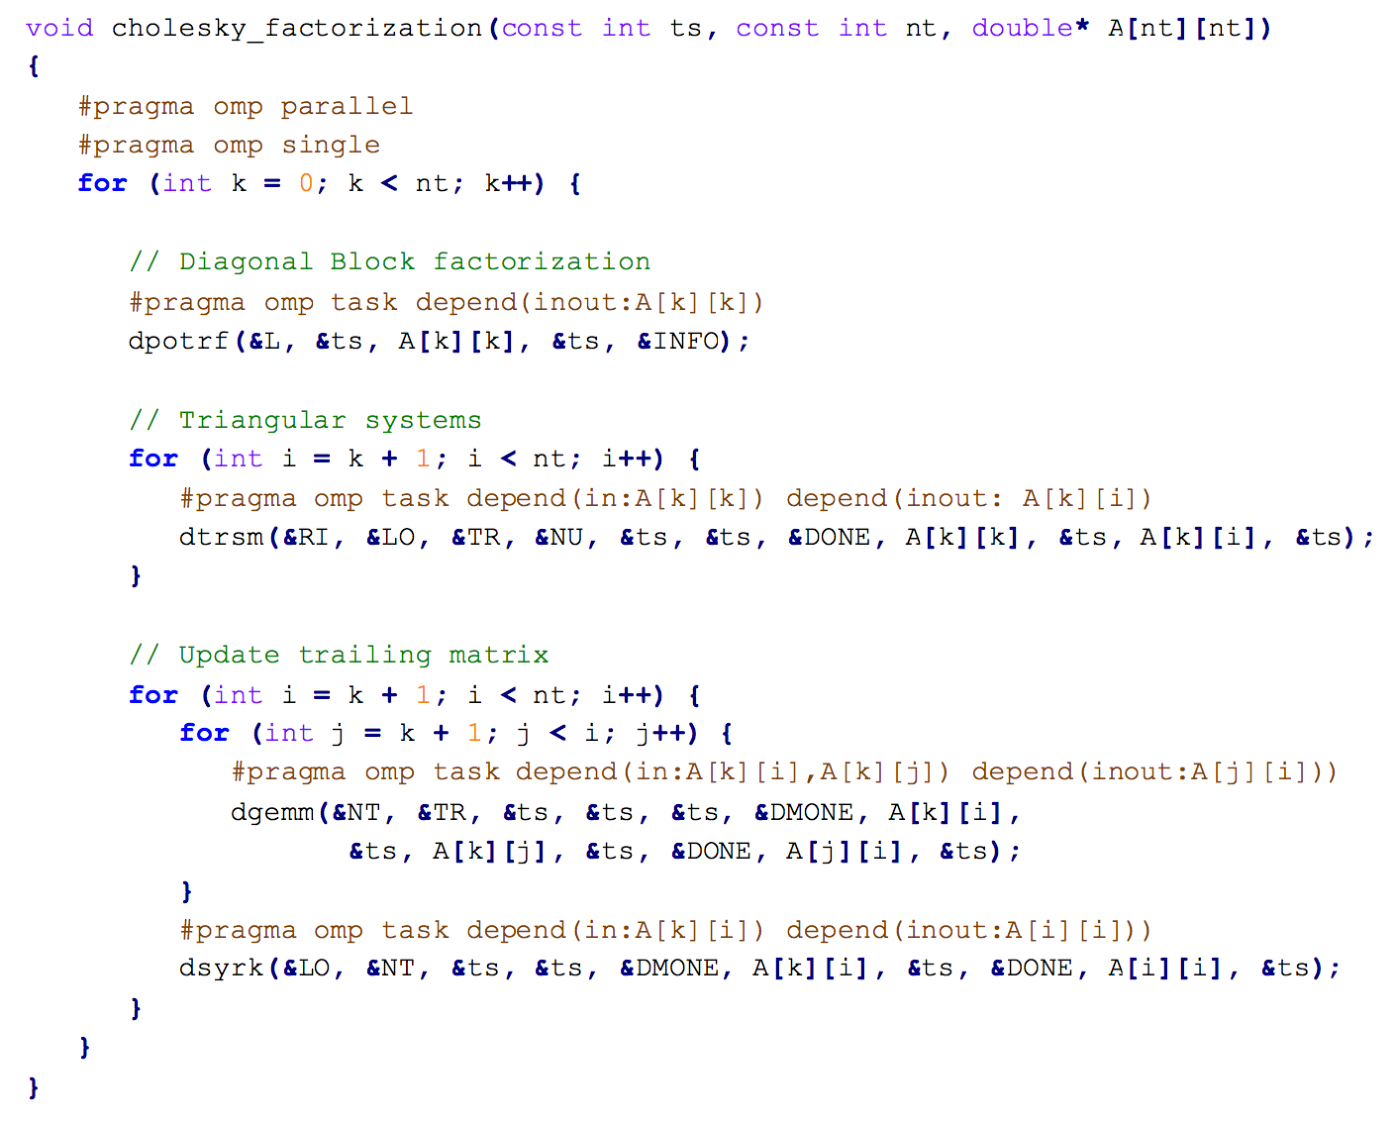
\includegraphics[width=0.85\textwidth]{images/cholesky}
      \caption{The Mixed Use of OpenMP Tasking and Intel MKL Library for Cholesky Factorization~\cite{intertwine}}
 \label{fig:cholesky}
\end{figure}


\subsubsection{Interoperability with inter-node programming model, e.g. MPI}
Hybrid parallel programming in the form of internode+intranode, e.g. MPI+X model are widely used for 
for high-performance computing. This approach reflects the two-level hierarchy of parallelism in current HPC systems, 
in which a high-speed interconnect
joins many highly parallel nodes.
Interoperability between inter-node programming model such as MPI and OpenMP 
systems has long been a productivity and composability goal within
the parallel programming community. We however still have not agreed on a standard solution from either of the two communities. 




%\subsubsection{OpenMP with native threads}
%\subsubsection{OpenMP with TBB/MKL}
%\subsubsection{OpenMP with parallel scientific library, such as MKL}
%\subsubsection{Linking libraries and objects built with different OpenMP compilers}
%\subsubsection{OpenMP with inter-node model, e.g. MPI}


\subsection{Issues with Poor Interoperability}
\subsubsection{CPU Oversubscription}
Oversubscription happens when resources are claimed and held than what is needed.
A program may request more OpenMP threads than the total amount of hardware
threads available when entering a parallel region, which causes excessive competition 
among OpenMP threads for hardware threads and increases runtime overhead. 
When program execution enters into sequential stage after exiting a parallel region, 
those native threads that support the OpenMP threads in the parallel region may still 
alive in the background consuming CPU cycles. This 
will make those hardware threads unavailable to others. 
Oversubscription impact the performance of an applications and the system, 
but should not introduce correctness issue to a program. 

%A typical OpenMP runtime creates a pool of native threads who will execute OpenMP
% parallel regions and/or tasks. 

The two scenarios we mentioned above are the two kinds of oversubscription we should try to avoid:
{\bf 1) Active oversubscription}: Claiming or requesting more threads than 
what are available by the system.
{\bf 2) Passive oversubscription}: Thread resources are not released 
after parallel execution. Holding hardware threads after parallel execution may not 
always hurt the performance overall, e.g. it will improve the start-up performance of the 
upcoming parallel region. In this category, we are concerning those situations that 
actually impact the performance negatively.



\subsubsection{Conflicting Thread Affinity}
Besides oversubscribing computational resources (hardwre cores) by an OpenMP program, 
memory and thread affinity are another kinds of resources that should be coordinately allocated and managed among
multiple parallel runtimes. %about how resources are utilized. 
Thread affinity conflict happens when an OpenMP runtime binds threads data to 
certain memory places (cache or NUMA region) that are already occupied by 
the affinity requests of another runtime. Such overlaps cause excessive cache or memory spills or relocation of data
to further places, resulting increased memory access latency becasue of false sharing or 
poor locality of thread and its data. %the places.
The affinity conflicts can happen even the total number of threads requested does not exceed the number of hardware threads available.
%Obviously, conflicting thread affinity may adversely impact the performance of programs involved. 



\subsubsection{Global Impact of Environment Variables}
The interoperability and composability of OpenMP programs are also limited by the global impact of OpenMP environment variables.
Currently, the OpenMP specification has an implicit assumption that a single OpenMP program is running on a computation node at any given time.
So the provided global environment variables should work properly to set the internal control variables that affect the execution
of the single OpenMP program. 
However, this causes problem when multiple OpenMP programs are running simultaneously on a computation node. 
Environment variables affecting resource allocation may uniformly impact all OpenMP programs, which is often not desired.
For example, unless runtime library routines are explicitly used to customize each program's choices, \lstinline{OMP_NUM_THREADS}, \lstinline{OMP_PROC_BIND}, \lstinline{OMP_DEFAULT_DEVICE} may 
make all OpenMP runtime instances use the same number of threads, the same affinity, and the same accelerator device, respectively. 



\subsection{Limitation of Interoperability Support in the Standard}
OpenMP currently (4.0) provides limited support for users to give hints to runtime for 
better managing OpenMP threads and native threads, which can be used to help reducing 
the impact of oversubscriptions.
\paragraph{OMP\_DYNAMIC} % environment variable}
This also includes dynvar ICV, omp\_set\_dynamic and omp\_get\_dynamic runtime routine. OMP\_DYNAMIC could be either
{\bf true} or {\bf false}. When setting the dynvar ICV to be {\bf true}, user will expect
OpenMP implementation to adjust the number of threads to use for executing parallel
regions in order to optimize the use of system resources.

\paragraph{OMP\_WAIT\_POLICY} %environment variable}
This also include waitpolicyvar ICV, but no getter and setter routine. 
OMP\_WAIT\_POLICY could be set as either ACTIVE or PASSIVE. 
The ACTIVE value specifies that waiting threads should mostly be active, consuming processor
 cycles, while waiting. An OpenMP implementation may, for example, make waiting threads spin.
 The PASSIVE value specifies that waiting threads should mostly be passive, not consuming
 processor cycles, while waiting. For example, an OpenMP implementation may make waiting
 threads yield the processor to other threads or go to sleep.
 The details of the ACTIVE and PASSIVE behaviors are implementation defined.
 
 \paragraph{OMP\_THREAD\_LIMIT}
 This also include threadlimitvar ICV and omp\_get\_thread\_limit getter runtime routine.
 The environment variable sets the maximum number of OpenMP threads to use in a contention group by setting the threadlimitvar ICV.
The behavior of the program is implementation defined if the requested value of OMP\_THREAD\_LIMIT is greater than the number of threads an implementation can support

OMP\_DYNAMIC and OMP\_THREAD\_LIMIT are approaches to
addressing active oversubscriptions, and OMP\_WAIT\_POLICY could be used to address
passive oversubscriptions. 
Since there are no setters for ICVs for OMP\_WAIT\_POLICY
and OMP\_THREAD\_LIMIT variable in the current standard, 
dynamically changing waiting policy and the maximum number of
threads at runtime is not available.

%\newpage

\section{Extensions to Address the Oversubscription Challenge}
\label{sec:proposal}

Most implementations of the parallel programming APIs rely on system 
native threading (PThreads or Windows Native threads) mechanisms to acquires system resources. 
Each implementation of the same or different APIs has its own mechanism and algorithms for managing
CPU resources. 
%OpenMP has been evolved to be a unified programming model for 
%parallel and heterogeneous computing nodes by including fork-join execution model, 
%data parallelism (worksharing), task parallelism, offloading execution model, etc.. 
%The runtime systems are becoming more complicated than before to support those language features.
A typical OpenMP runtime maintains 
an internal thread pool to keep track of the native threads created by the runtime even they are not  
doing any OpenMP operation during the sequential execution of the program. 
In the fork-join OpenMP execution model, a native thread in the thread pool 
is summoned to participate in an OpenMP team for computation upon the fork of the {\sf parallel} region. 
The native thread returns back to the thread pool when a parallel 
region is finished at the join barrier. While in the 
thread pool, a native thread blocks in a fork barrier. 
OpenMP runtime may also
%Instead of moving the blocking thread to the thread pool, 
maintains internal hot teams that keep threads actively waiting for the upcoming parallel regions. 
%in which threads are busy-waiting for work even if the program is in the sequential stage. 
So an OpenMP program could consumes cycles of multiple CPU cores even if it is in sequential execution stage.

It is also often that an OpenMP program explicitly create native threads, e.g. PThreads, and each native thread has
its own OpenMP {\sf parallel} region. 
In such hybrid user-level native thread/OpenMP program, e.g. 
a runtime may form an internal decendant hierarchy for the native threads created by users and
those by the OpenMP runtime. Borrowing the terms from Intel OpenMP runtime implementation, we refer to 
the native threads created by users as root threads. 
In the most recent OpenMP standard, a root thread forms a contention group and we thus 
consider all the decedant threads are members of the contention group. 


The oversubscription challenge is then concerned with how 
to coordinate the CPU resource sharing between two or more contention groups, and between multiple 
runtime instances, which could be of the same or different runtime libraries. 
Our solutions for addressing it provide users APIs for 
dynamically setting the waiting policy of the blocking thread to minimize 
the consumption of CPU cycles when idling. 
%so threadsthat do not do useful work consume minimum CPU cycles. 


\subsection{Definition of the ACTIVE and PASSIVE Wait Policies}
Our proposal defines more specifically 
the ACTIVE and PASSIVE policies and also extends each to include multiple policies that dictate more
specifically the exact behavior of the waiting thread. 
When a thread is waiting in ACTIVE state, it should not initiate calls to
relinquish the CPU, though technically the OS kernel or hardware may switch it out of the core it occupies. 
When in PASSIVE state, a thread initiates yielding or suspension operation to give up the CPU core. 
The extensions of each of the policies are summerized in Table~\ref{table:implement_wait} and detailed description
follows the table. 
\begin{table}[ht]
	\centering
\resizebox{12.5cm}{!}{
\begin{tabular}{|l|l|l|l|}
\hline
\multicolumn{2}{|c|}{\textbf{Wait Policy}} & \textbf{Description} & \textbf{Pseudo code} \\
\hline
\multirow{2}[4]{*}{{ACTIVE}} & {SPIN\_BUSY} & Busy wait in user level & while (!finished()) ; \\
\cline{2-4}      & {SPIN\_PAUSE} & Busy wait while pausing CPU & while (!finished()) cpu\_pause() \\
\hline
\multirow{3}[6]{*}{{PASSIVE}} & {SPIN\_YIELD} & Busy wait with yield & while (!finished()) sched\_yield(); \\
\cline{2-4}      & {SUSPEND} & Thread sleeps. Others wake it up. & mutex wait(); mutex wake(); \\
\cline{2-4}      & {TERMINATE} & Thread terminates &  \\
\hline
\end{tabular}%
}
\label{table:implement_wait}
\caption{Wait Policies}
\end{table}

%The blocking mechaims could be  
%either busy-waiting which occupies a CPU core, or in the kernel
%scheduling queue after a yield system call (e.g. {\em sched\_yield} in Linux), or could be put to sleep. 
%thread could be in one of the following states while not participating in OpenMP computations.  
	{\bf ACTIVE SPIN\_BUSY}: The blocking thread spins waiting in a loop purely in user space. 
%		It is released from the barrier to participate in a team for computation by the runtime. 
		It consumes CPU cycles and memory bandwidth while loop checking
		the condition for being released. This policy allows the fastest response time when a thread is
		released from the barrier. 

	{\bf ACTIVE SPIN\_PAUSE}: The blocking thread spins waiting using a loop and also pauses the CPU core in 
	each loop iteration. The pause operation introduces a slight delay in the loop, reducing the amount 
	of instructions fed into the pipeline as well as the energy consumption. This policy also allows 
	for very fast response time but consuming much less amount of CPU cycles 
	and memory bandwidth than the SPIN\_BUSY policy.

	{\bf PASSIVE SPIN\_YIELD}:  The blocking thread spins waiting using a loop and 
	relinquishs the CPU in each iteration by kernel system call (e.g. {\em sched\_yield}). CPU yielding causes
	the thread to be moved to the end of the kernel scheduling queue for its static priority. A thread in this 
		stage can only be released to the OpenMP runtime by the kernel. Kernel context switch is involved
		in each loop iteration, thus having higher overhead than the two ACTIVE policies. 
		This policy provides average response time, but allows kernel to schedule other tasks to the same
		CPU core while the thread yields. 

	{\bf PASSIVE SUSPEND}: The thread is suspended when waiting in the barrier call. A suspended thread can only
	be resumed by other threads, being timed out, or upon some hardware state change~\footnote{
                    On Intel platforms, this can be implemented using {\em monitor-mwait}.
                    Blue Gene/Q supported a ``wake-up unit'' for fast thread resumption.
                     Other processors may have similar features.}. A suspended thread, also known as sleeping,  
		     does not consume CPU cycles. 
		     However the operations of suspending or resuming a thread are costly. 
		     Thus this approach has the longest response time and 
		     the kernel can completely allocate other tasks to the CPU 
		     core previously used by the thread that is suspended now.

       {\bf PASSIVE TERMINATE}: The thread will be terminated instead of waiting in the runtime. Though not technicall accurate as
       a ``waiting" policy, it is categorized as the PASSIVE policy because of the same effect of it as the {\sf PASSIVE SUSPEND} policy. 
       By introducing this policy, 
       we give users an option to return completely the CPU cores to the system, though the future request of thread requires to
       recreating the thread. The termination and recreation of a thread cost more than suspending and resuming a thread.  

\subsection{Proposed Runtime Routines} 
%This interoperability proposal is an effort from OpenMP interoperability language subcommittee for addressing
%the oversubscription challenges of OpenMP programs when being executed with other threading library. 
Our extensions to OpenMP are runtime routines that can explose 
certain functionalities of the runtime systems for users to 
intrusively adjust the behavior of the waiting threads.  
%These routines  API for providing more information or control to users 
%for the threads in the runtime, 
They also include routines for the runtime to contribute OpenMP threads for another parallel runtime, without
the need to create a {\sf parallel} region. The specifications are included in the follow list. 
%Parallel programming models such as 
%The proposal introduces the following definition of data types and runtime routines. 

\lstset{basicstyle=\sffamily\small,language=c, numbersep=1pt}
\begin{lstlisting}[frame=single]  % Start your code-block

typedef enum omp_wait_policy {
  OMP_SPIN_BUSY_WAIT = 1,  /* 0x1 */
  OMP_SPIN_PAUSE_WAIT = 2, /* 0x10 */
  OMP_SPIN_YIELD_WAIT = 4, /* 0x100 */
  OMP_SUSPEND_WAIT = 8,    /* 0x1000 */
  OMP_TERMINATE = 16, /* 0x10000 */

  OMP_ACTIVE_WAIT = OMP_SPIN_PAUSE_WAIT,
  OMP_PASSIVE_WAIT = OMP_SUSPEND_WAIT;
} omp_wait_policy_t; 

int omp_get_num_threads_runtime(omp_wait_policy_t state);

void omp_set_wait_policy(omp_wait_policy_t wait_policy);
int omp_get_wait_policy(void);

int omp_quiesce(omp_wait_policy_t state);

typedef void * omp_thread_t;
int omp_thread_create (omp_thread_t * th, int place,  
   void *(*start_routine)(void *), void *arg, void * new_stack);
void omp_thread_exit(void *value_ptr);
int omp_thread_join(omp_thread_t thread, void **value_ptr);

\end{lstlisting}
The {\sf omp\_wait\_policy\_t} enum defines the valid thread waiting policies that can be passed to the 
related runtime routines. The value for {\sf OMP\_ACTIVE\_WAIT} and {\sf OMP\_PASSIVE\_WAIT} could be defined
in the standard. It is also posibble that the standard does not define the five specific policies, and let 
the implementers specify the meaning of ACTIVE or PASSIVE policies in their implementation. The use of the binary
position bit (0x1, 0x10, etc) allows for setting multiple wait policies for a thread such that the thread can automatically change
its waiting behavior according to the needs of the application. 
%to be defined by the
%implementers who will  


%We use those state as the waiting policy that a user would want the runtime threads to be in and the 
\subsection{The {\sf omp\_get\_num\_threads\_runtime} Runtime Routine}
This routines return the number of runtime threads that are under the specified policy. The binding thread set 
of the function is the team threads when being called inside a parallel region, and all the threads in the current 
contention group when being called in the sequential region. The information provided by calls to this routines can be used 
by users to make resource management decision when oversubscription become an issue in a program. 

\subsection{The {\sf omp\_set\_wait\_policy} and {\sf omp\_get\_wait\_policy} Runtime Routines}
The {\sf omp\_set\_wait\_policy} runtime setter routine sets wait policy of binding thread(s). 
%It is important to note that the call to this routine impacts differently for 
When being called inside a {\sf parallel} region, the routine sets the wait policy of the calling thread. 
%the master thread will make changes of the wait policy for all the team threads. 
When being called in a sequential region, the routine sets the wait policy for all the 
d threads of the binding contention group. The {\sf omp\_get\_wait\_policy} routine returns the wait policy 
of the binding thread if it is being called inside a {\sf parallel} region. If being called in a sequential region, 
this getter routine returns the wait policy of the contention group if the policy is set before by the setter. 
If no wait policy has been set for the contention group by the setter, the getter routine returns the wait policies 
of all the threads as a combined integer. For example, the return value of 0x1011 indicates that OMP\_SUSPEND\_WAIT, 
OMP\_SPIN\_PAUSE\_WAIT and OMP\_SPIN\_BUSY\_WAIT policies have been set for the threads of the contention group. The
difference of the binding thread set according to where the setter is called (a {\sf parallel} region or sequential region) 
allows users to set the policies of the selected threads in a contenton group. For example, the {\sf omp\_set\_wait\_policy(OMP\_PASSIVE\_WAIT)} 
call in the sequential region followed by the {\sf omp\_set\_wait\_policy(OMP\_ACTIVE\_WAIT)}  
call inside a {\sf parallel} region enable the setting of those threads that are not part of the {\sf parallel} region to be PASSIVE waiting while
other threads should be ACTIVE waiting. 
%The valid arguments for this call 
%include {\sf omp\_thread\_state\_SPIN}, {\sf omp\_thread\_state\_YIELD}, 
%and {\sf omp\_thread\_state\_SLEEP}. The value of  {\sf OMP\_ACTIVE\_WAIT} and 
%{\sf OMP\_PASSIVE\_WAIT} could be implementation or language defined. 
The setter call makes changes of the wait policy to invidual threads, thus thread waiting behavior overrides the default 
setting by the wait-policy-var ICV and OMP\_WAIT\_POLICY environment variables. 

The {\sf omp\_set\_wait\_policy} routine can be used for addressing both active and passive oversubscription depending the location of the call to 
this routine. It is also important to note that compilers from IBM, Cray and Oracle have provide similar feature~\cite{ibmwait,craywait,oraclewait}.
There are also different variants of this features depending how much details users can configure
the wait policy. For example, Oracle OpenMP runtime allows users to set policies for specific execution point, e.g, at OpenMP 
barrier or after a parallel region. 

\subsection{The {\sf omp\_quiesce} Runtime Routine}
The {\sf omp\_quiesce} routine quiesces all OpenMP threads of the runtime according to 
specified threading behavior by the argument, which could be either OMP\_SUSPEND\_WAIT or OMP\_TERMINATE. The binding thread set include
all the threads of the runtime instance. 
%SLEEP or KILL. 
Thus quiescence involves termination of threads or otherwise inactivating them. 
The routine returns zero if quiescence has been achieved, otherwise it returns a non-zero error code.

%The two APIs allow a program to dynamically change the behavior of waiting threads or even shutdown the runtime, thus addressing the passive
%oversubscription issue. 


\subsection{The {\sf omp\_thread\_create/exit/join} Runtime Routines}

The {\sf omp\_thread\_create/exit/join} APIs are for creating OpenMP threads similarly as user threads such 
as PThreads. The {\sf place} parameter is used for specifying the place where the thread should be created from.  
By using those APIs, an OpenMP thread
can be used as regular thread without using OpenMP parallel region. Those threads can be used to form another parallel runtime for other programming
models, but also being tracked by the OpenMP runtime, but not belong to any thread team. 


\REM{
with one of the thread state. This will allow programmers to explicitly change the policy at various 
points during a program's execution. An efficient implementation may use atomic write to the 
global ICV and all threads will react accordingly at some later point of the execution after the 
ICV is set. So the effects may be delayed. 
The {\sf omp\_set\_wait\_policy} should only make effects to threads created from the current root thread 
of the runtime when the parameter is one of the three:
{\sf omp\_thread\_state\_WAIT} which corresponds to the {\sf ACTIVE} wait policy, 
{\sf omp\_thread\_state\_YIELD} which corresponds to the {\sf PASSIVE} wait policy, or
{\sf omp\_thread\_state\_SLEEP}. 
%The {\sf ACTIVE} for {\sf OMP\_WAIT\_POLICY} environment variable is the same as 
%the {\sf omp\_thread\_state\_WAIT}, and the {\sf PASSIVE} is the same as the {\sf omp\_thread\_state\_YIELD}.



%, for processing tasks such as message passing that are not computational, or for receiving
%help from user threads to do OpenMP work. We also observed that a highly-interoperable OpenMP proposal is 
%complex for both the usage and implementation of those features. It introduces
%overheads that may not be necessary for a program that does not need to interoperate in that degree of interoperability. 
Thus we categorize interoperability functionalities into the following multiple levels: 
\begin{itemize}
	\item {\bf Level 0, OMP\_INTEROP\_NONE}: No interoperability. The OpenMP runtime does not provide mechanism to interoperate with others.
	\item {\bf Level 1, OMP\_INTEROP\_INFORM}, Informational. Constructs for providing information for others about the internal status of the thread pool, thread affinity info, etc. 
	\item {\bf Level 2, OMP\_INTEROP\_SELF}: Self adjusting threading behavior. Constructs for
		externals to use to adjust its internal threading and affinity behaviors.
	\item {\bf Level 3, OMP\_INTEROP\_CONTRIBUTE}: Contributing. Constructs for externals to use to acquire OpenMP 
		threads or places for doing user-specific tasks that are not part of the OpenMP. It also includes constructs for injecting
		a user-specific task into the runtime. 
	\item {\bf Level 4, OMP\_INTEROP\_REAP}: Receiving help. Constructs for externals to attach user threads into the runtime.
\end{itemize}

In each level, 
OpenMP constructs (directives, runtime APIs and environment variables) are defined to support the interoperability 
requirements. 
An OpenMP implementation that supports a certain level of interoperability should provide the implementation of all the APIs
from level 0 to that level inclusively. 
An environment variable, {\sf OMP\_INTEROP\_LEVEL}, is defined to set the desired level of 
interoperability for an OpenMP program. The actual level during execution depends on both the value of 
the variable and the level which the implementation supports. 
The ``{\sf int omp\_get\_interop\_level()}" procedure should be provided for querying the current level. % being supported by an OpenMP runtime. 
%An OpenMP implementation supports the desired level of interoperability and should 

\subsection{Level 0, OMP\_INTEROP\_NONE}
In this level, an OpenMP runtime should be independent from others, even when there are multiple instances of the same runtime library. 
%An OpenMP runtime instance should be created for each user thread that launch 
%into OpenMP functions. 
The thread behavior, e.g. wait policy, thread-limit, dynamic cannot be changed after the runtime started.
The runtime takes the values of those variables from environment variables. The implementation supporting 
this level should implement the following  
environment variables and some getter functions. 
\lstset{basicstyle=\sffamily\footnotesize,language=c, numbersep=1pt}
\begin{lstlisting}[frame=single]  % Start your code-block

OMP_DYNAMIC                     /* in the standard already */
OMP_WAIT_POLICY                 /* in the standard already */
OMP_THREAD_LIMIT                /* in the standard already */
int omp_get_dynamic(void);      /* in the standard already */
int omp_get_thread_limit(void); /* in the standard already */
int omp_get_wait_policy(void);
int omp_get_num_procs(void);    /* in the standard already */

typedef struct omp_thread omp_thread_t;
omp_thread_t * omp_get_initial_thread();

typedef struct omp_runtime_handle omp_runtime_handle_t;
omp_runtime_handle_t omp_get_runtime_handle();
\end{lstlisting}
The {\sf omp\_get\_wait\_policy} implementation should return the value set by the environment. 
As we mentioned that environment setting impacts all the runtime instances by setting the corresponding
ICVs of each runtime the same values. For helping setting runtime-specific ICVs if a setter is available, a program
can use the {\sf omp\_get\_initial\_thread} and {\sf  omp\_get\_runtime\_handle} to retrieve the handle for the
initial thread and a runtime handle. However, a runtime instance can only set the ICVs for its own. 

\subsection{Level 1, OMP\_INTEROP\_INFORM}
This level defines APIs for users to query the internal status of the runtime, including the size of thread pool, the number of threads
that are busy-waiting, yielding or sleeping. The status of a thread includes RUN, WAIT, YIELD, SLEEP, KILL, and BLOCK. 

\lstset{basicstyle=\sffamily\small,language=c, numbersep=1pt}
\begin{lstlisting}[frame=single]  % Start your code-block

typedef enum omp_wait_policy {
  omp_wait_policy_RUN = 0,     /* doing useful work */
  omp_wait_policy_WAIT = 1,    /* busy waiting for work */
  omp_wait_policy_YIELD = 2,   /* yield the CPU */
  omp_wait_policy_SLEEP = 3,   /* sleeping */
  omp_wait_policy_KILL = 4,    /* being killed */
  omp_wait_policy_BLOCK = 5,   /* blocked waiting */
} omp_wait_policy_t; 
int omp_get_num_threads_runtime(omp_wait_policy_t state);
\end{lstlisting}

By using the API, a program would be able to claims or allocate appropriate amount of resources based on how many are occupied by the OpenMP
runtime to avoid active oversubscription. 

\subsection{Level 2, OMP\_INTEROP\_SELF} 
In this level, APIs are defined for adjusting the runtime behavior of the runtime, including the wait policy, dynamic feature, etc.

\begin{lstlisting}[frame=single]
void omp_set_dynamic(int dyn_threads); /*in standard already*/
void omp_set_wait_policy(omp_wait_policy_t wait_policy);
int omp_quiesce(omp_wait_policy_t state);
\end{lstlisting}
The {\sf omp\_set\_dynamic} is already in the standard. 

The {\sf omp\_quiesce} routine quiesces all OpenMP threads of the runtime according to specified threading behavior by the parameter. The
parameter could be either WAIT, YIELD, SLEEP, or KILL. Quiescence may involve termination
 of threads or otherwise inactivating them. The routine returns zero if quiescence has been achieved, otherwise it returns a non-zero error code.

The two APIs allow a program to dynamically change the behavior of waiting threads or even shutdown the runtime, thus addressing the passive
oversubscription issue. 


\subsection{Level 3, OMP\_INTEROP\_CONTRIBUTE}
The APIs in this level mean to contribute the resources owned by an OpenMP runtime to externals. 
% for operations that are not easy to describe using OpenMP directives.  

\lstset{basicstyle=\sffamily\small,language=c, numbersep=1pt}
\begin{lstlisting}[frame=single]  % Start your code-block

int omp_thread_create (omp_thread_t * th, int place,  
   void *(*start_routine)(void *), void *arg, void * new_stack);
void omp_thread_exit(void *value_ptr);
int omp_thread_join(omp_thread_t thread, void **value_ptr);

typedef struct omp_task omp_task_t;
void omp_task_create(omp_task_t * t, void *(*task_func)(void *), 
  void * task_args, int (*task_test_func)(omp_task_t), 
  int *intags, int num_intags, int * outtags, int num_outtags);
\end{lstlisting}
The {\sf omp\_thread\_create/exit/join} APIs are for creating OpenMP threads similarly as user threads such 
as PThreads. The {\sf place} parameter is used for specifying the place where the thread should be created from.  
By using those APIs, an OpenMP thread
can be used as regular thread without using OpenMP parallel region. Those threads can be used to form another parallel runtime for other programming
models, but also being tracked by the OpenMP runtime, but not belong to any thread team. 

The {\sf omp\_task\_create} procedure allows users to inject non-blocking tasks into the OpenMP runtime. A non-blocking task does not occupy
a thread during the execution, it only requires the runtime to launch the task and to periodically query the task internally. The non-blocking
tasks will be part of a {\sf taskgroup}, or joining a {\sf taskwait} or {\sf barrier} synchronization. It can be used with task dependencies by 
passing the tags for in and out dependency. A typical use case for this API is to request OpenMP runtime to launch a non-blocking MPI call by providing the call information and a function pointer for query the completion of this task. Again, runtime only launches the tasks and then periodically
query its status using the provided {\sf task\_test\_func} function pointer parameter of {\sf omp\_thread\_create}.

\subsection{Level 4, OMP\_INTEROP\_REAP} 
The philosophy of this level of interoperability support is to enable an OpenMP runtime to accept offer of threads 
for helping its own execution. This is different than the approach of claiming CPU cores 
for computation using the standard parallel region creation. By allowing program to offer threads to the runtime who needs it, we are able to 
reap the resources for computation, thus reducing the overhead of thread creation and context switching when otherwise 
a thread has to be terminated from
one runtime and then recreated in another runtime in order to use the same core. 
\lstset{basicstyle=\sffamily\small,language=c, numbersep=1pt}
\begin{lstlisting}[frame=single]  % Start your code-block

int omp_thread_attach(omp_runtime_handle_t runtime, 
    void * new_stack, int place, int * term_flag);
\end{lstlisting}

The {\sf omp\_thread\_attach} procedure accepts a parameter for specifying a new stack for the thread when it joins the runtime. It also 
allows for specifying a target place the thread should bind to. 
The {\sf term\_flag} 
is used for signaling the runtime that the attached thread should terminate when the variable becomes true. 
The runtime evaluates the {\sf term\_flag} when the thread is not performing OpenMP work. 



There are still some challenges in terms of OpenMP interoperability. 
OpenMP threads that are created by the parallel construct cannot interact with external systems. 
In other words, we are trying to enable the interoperability through flexible communication between OpenMP threads and user threads. 
However, the main goal of this work is to achieve a high level of resource utilization. So, it would be better if OpenMP threads can interact and communicate with user threads. To achieve this goal, we implement four new functions as follows:
\begin{enumerate}
	\item int omp{\_}set{\_}wait{\_}policy(ACTIVE \textbar PASSIVE): 
	set the waiting thread behavior. The function returns the current wait{\_}policy, which could be different from intention of the call depending on the decision made by the runtime. If the value is PASSIVE, waiting threads should not consume CPU power while waiting; while the value is ACTIVE specifies that they should.
	\item int omp{\_}thread{\_}create( ): 
	to give the user the ability to create an OpenMP thread without using \#pragma omp parallel directive, and lets it be a user thread similar to pthread.
	\item int omp{\_}quiesce( ): 
	to shutdown or unload the OpenMP runtime library.
\end{enumerate}
}


\section{Implementation and Evaluation}
\label{sec:implementation}
The ongoing implementation was performed in both Intel OpenMP runtime (iOMP) and GNU Compiler Runtime (GOMP). The implementations for 
the constructs for Level 0 and 1 are straightforward since they all for exposing the internal status of the runtime. In this section, 
we highlight the implementation and evaluation of some of the functions in Level 2 and 3: 
{\sf omp\_set\_wait\_policy}, {\sf omp\_quiesce} and {\sf omp\_thread\_create/exit/join}. 
In general, to implement those four functions, we follow the three steps:
\begin{itemize}
	\item Define this function in file “kmp{\_}csupport.c”, 
	write down the implementation.
	\item Declare this function in file “kmp.h”, 
	using “KMP{\_}EXPORT” in front the declaration.
	\item Export this function in file “dllexports”, 
	assign a unique ID for this function.
\end{itemize}

\begin{enumerate}
	\item void omp{\_}quiesce()
	
	The purpose of this function is to shutdown or destroy all OpenMP threads in the thread pool. We have implemented it, as shown in Figure~\ref{omp:quiesce}, by using the Intel internal call to {\_}kmp{\_}internal{\_}end{\_}fini, which unloads the runtime library. Then, we have to register the master thread again so it can generate team of threads later when needed. This can be done by calling the {\_}kmp{\_}get{\_}global{\_}thread{\_}id{\_}reg( ).
	
	\begin{figure}
		\centering
		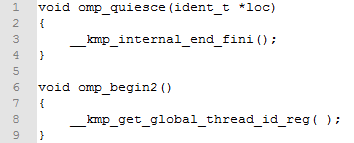
\includegraphics[width=0.7\textwidth] {images/omp_quisce}
		\caption{omp\_quiesce}
		\label{omp:quiesce}
	\end{figure}
	
	\item void omp{\_}set{\_}wait{\_}policy(PASSIVE \textbar ACTIVE)
	
	The idea of this function is to set the waiting thread behavior. PASSIVE value means that waiting threads should not consume CPU power while waiting. In other words, the OpenMP runtime system will put them into a sleep mode. On the other hand, ACTIVE value means that waiting threads should keep asking the CPU for work to do. The intention of doing this function is to measure the differences in performance between these different modes. 
	The implementation of this function is done by using the internal {\_}kmp{\_}stg{\_}parse{\_}wait{\_}policy as shown in Figure~\ref{omp:set_wait_policy}. The current OpenMP runtime system uses the library{\_}turnaround to indicate the ACTIVE mode and library{\_}throughput to indicate the PASSIVE mode. We pass an integer as its parameter. If it equals to 0, we set the wait policy to be passive, otherwise, active. We found a variable named “{\_}kmp{\_}library” in the environment setting file which has four different status for the waiting policy. So, we change this value accordingly, then we call a function “{\_}kmp{\_}aux{\_}set{\_}library” to set the changed value to the OpenMP environment.
	
	\begin{figure}
		\centering
		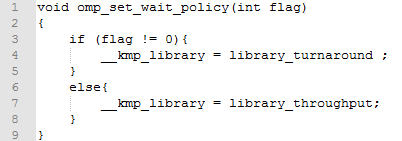
\includegraphics[width=0.7\textwidth] {images/omp_set_wait_policy}
		\caption{omp\_set\_wait\_policy}
		\label{omp:set_wait_policy}
	\end{figure}
	
	\item int omp{\_}thread{\_}create()
	
	The purpose of this function is to give the user the ability to create an OpenMP thread without using \#pragma omp parallel directive, and lets it be a user thread similar to pthread. The implementation of this function is shown in Figure~\ref{omp:create_thread}.
	So, we are creating one thread to execute the passed function. If there are enough available threads in the thread pool, we will get one thread from the thread pool and assign the task to it. If no thread is available in the thread pool, we create a new thread to execute this task, and then put the new thread back into the thread pool after completing its job. 
	
	\begin{figure}
		\centering
		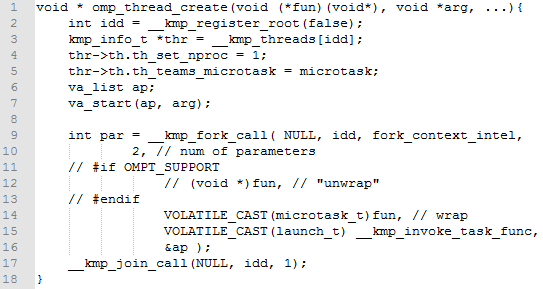
\includegraphics[width=0.7\textwidth] {images/omp_create_thread}
		\caption{omp\_create\_thread}
		\label{omp:create_thread}
	\end{figure}
	
\end{enumerate}

\subsection{Evaluation}
\label{sec:results}
The evaluation was performed on a machine using two Intel(R) Haswell-EP Xeon(R) E5-2699v3 processors with total 36 cores supporting 72 threads. We use the latest
LLVM compiler version 3.8.0 for evaluating IOMP implementation. Test programs were designed to evaluate the overhead of these functions. 
%\subsubsection{{\sf omp\_quiesce}}

We first developed microbenchmarks for evaluating parallel startup cost after applying different wait policy or 
quiescing the runtime system, as well as the cost for the {\sf omp\_set\_wait\_policy} and {\sf omp\_quiesce} 
routines.  
Figure~\ref{omp:overhead_table} shows the results of the evaluation. 
The use of each of the two {\sf ACTIVE} policies and the PASSIVE(SPIN\_YIELD) policy 
introduce very minimum and neglectable overhead to the {\sf parallel} region startup. 
When PASSITVE(SUSPEND) policy is applied, we observed significant increase of overhead of creating parallel region, 
which can be explained by the cost to suspend and resume the runtime threas when the policy is in effect. 
The use of {\sf omp\_quiesce} with TERMINATE policy, which completely shutdown the 
runtime, dramatically increase the overhead, close to 1000x, of starting the a new parallel region. In this 
scenario, the cost of initializing the whole runtime is counted toward {\sf parallel} startup overhead. Second, 
for the overhead of the two routines, {\sf omp\_set\_wait\_policy} incurs very minimum overhead. The 
{\sf omp\_quiesce} routine however incurs high overhead since it needs to terminate the runtime threads as well as 
destroy all the resources allocated for the runtime (e.g. mutex, condition variables and memory, etc). 

%The overhead evaluations show that the ACTIVE(SPIN) and YIELD policies do not impact much of the {\sf parallel} 
%region start up. The PASSIVE(SLEEP) policies introduce overheads for creating new parallel regions that need to wake up sleeping thread, thus should use with care. The {\sf omp\_quiesce(KILL)} is a heavy operations and should only be
%used when there is no need to use the runtime in the program. 

%The test measures the overhead of starting 
%up an OpenMP runtime and shutting down a runtime by using {\sf omp\_quiesce}, as compared to creating a parallel region. 
%The cost of creating a parallel region is very light because of the use of internal hot teams maintained by the runtime. 
%The cost of shutting down the runtime is about half of the cost of starting a runtime, 
%but about 4 to 10 times of the cost of parallel region creation. 

\begin{figure}[ht]
    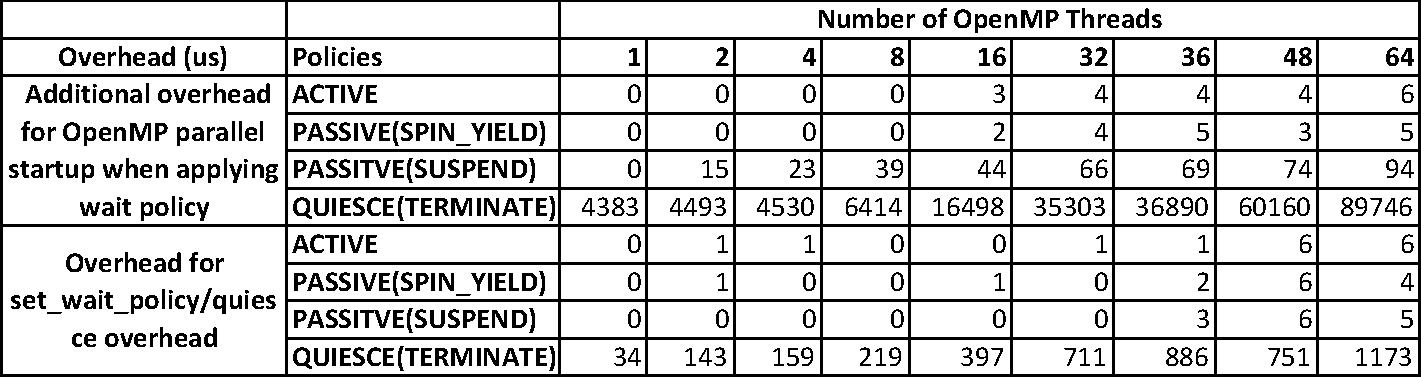
\includegraphics[width=0.99\textwidth] {images/parallel_set_quiesce_overhead}
    \caption{Overheads for OpenMP parallel and for {\sf omp\_set\_wait\_policy} and {\sf omp\_quiesce} implementation}
    \label{omp:overhead_table}
\end{figure}

\REM{
\begin{figure}[ht]
    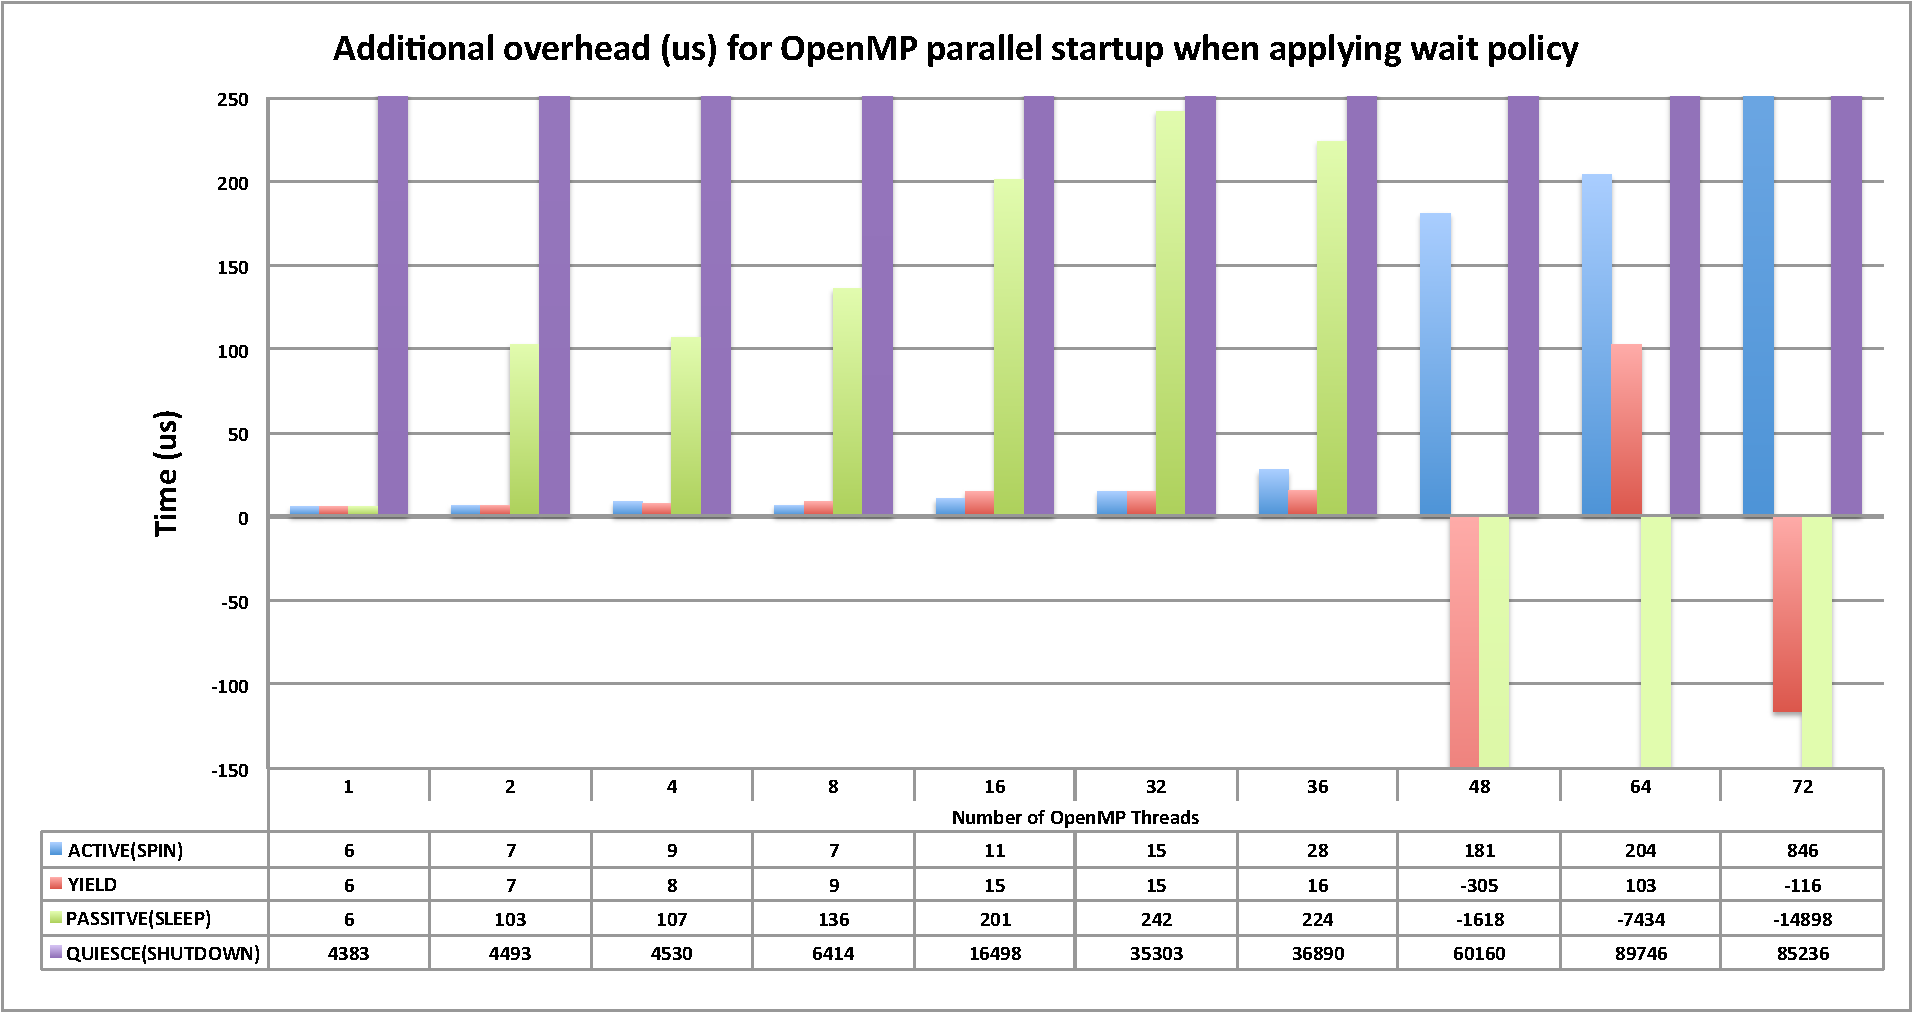
\includegraphics[width=0.99\textwidth] {images/parallel_overhead}
    \caption{Additional Overheads (us) for OpenMP parallel when applying {\sf omp\_set\_wait\_policy} and {\sf omp\_quiesce}}
    \label{omp:parallel_overhead}
\end{figure}
}

Our next evaluation was designed to measure the execution time of hybrid PThread/OpenMP program when different
wait policies are applied. We develop a program in which multiple PThreads are created, 
each of which executes the funciton shown in the following list. 
Each PThread first spins waiting for a specific period of time, and  
then enters into a parallel region in which perform busy-waiting for 3000 us.
The time periods of the two busy waiting (one is sequential and one is parallel) are carefully designed for
all PThreads so theoritically only one PThread enters into parallel region a time. The 
OpenMP threads for each PThread are scheduled by the kernel onto the available 
cores. When there are enough cores to support all threads (including the PThreads and OpenMP threads),
which means no oversubscription, mininum scheduling overhead and context switch are incurred, thus the optimal 
performance. In this test case, we define two crosspoints. The first crosspoint (\#1) is when the oversubscription
over the total number of cores in the test system (36 cores) happens and the second one (\#2) is when the oversubscription
over the total number of hardware threads (72) happends. 


\lstset{basicstyle=\sffamily\footnotesize,language=c, numbersep=1pt}
\begin{lstlisting}[frame=single]  % Start your code-block

void *omp_parallel_foo(void *ptr ) {   
    int user_thread_id = (int) ptr;
    for (int i=0; i<NUM_ITERATIONS; i++) {
        /* busy wait befor entering parallel region */
        busy_waiting(user_thread_id*3000);
#pragma omp parallel num_threads(num_ompthreads)
        {   
            busy_waiting(3000); /* act as computation */
        }
        omp_set_wait_policy(policy);
    }
}

\end{lstlisting}


\begin{figure}[h]
    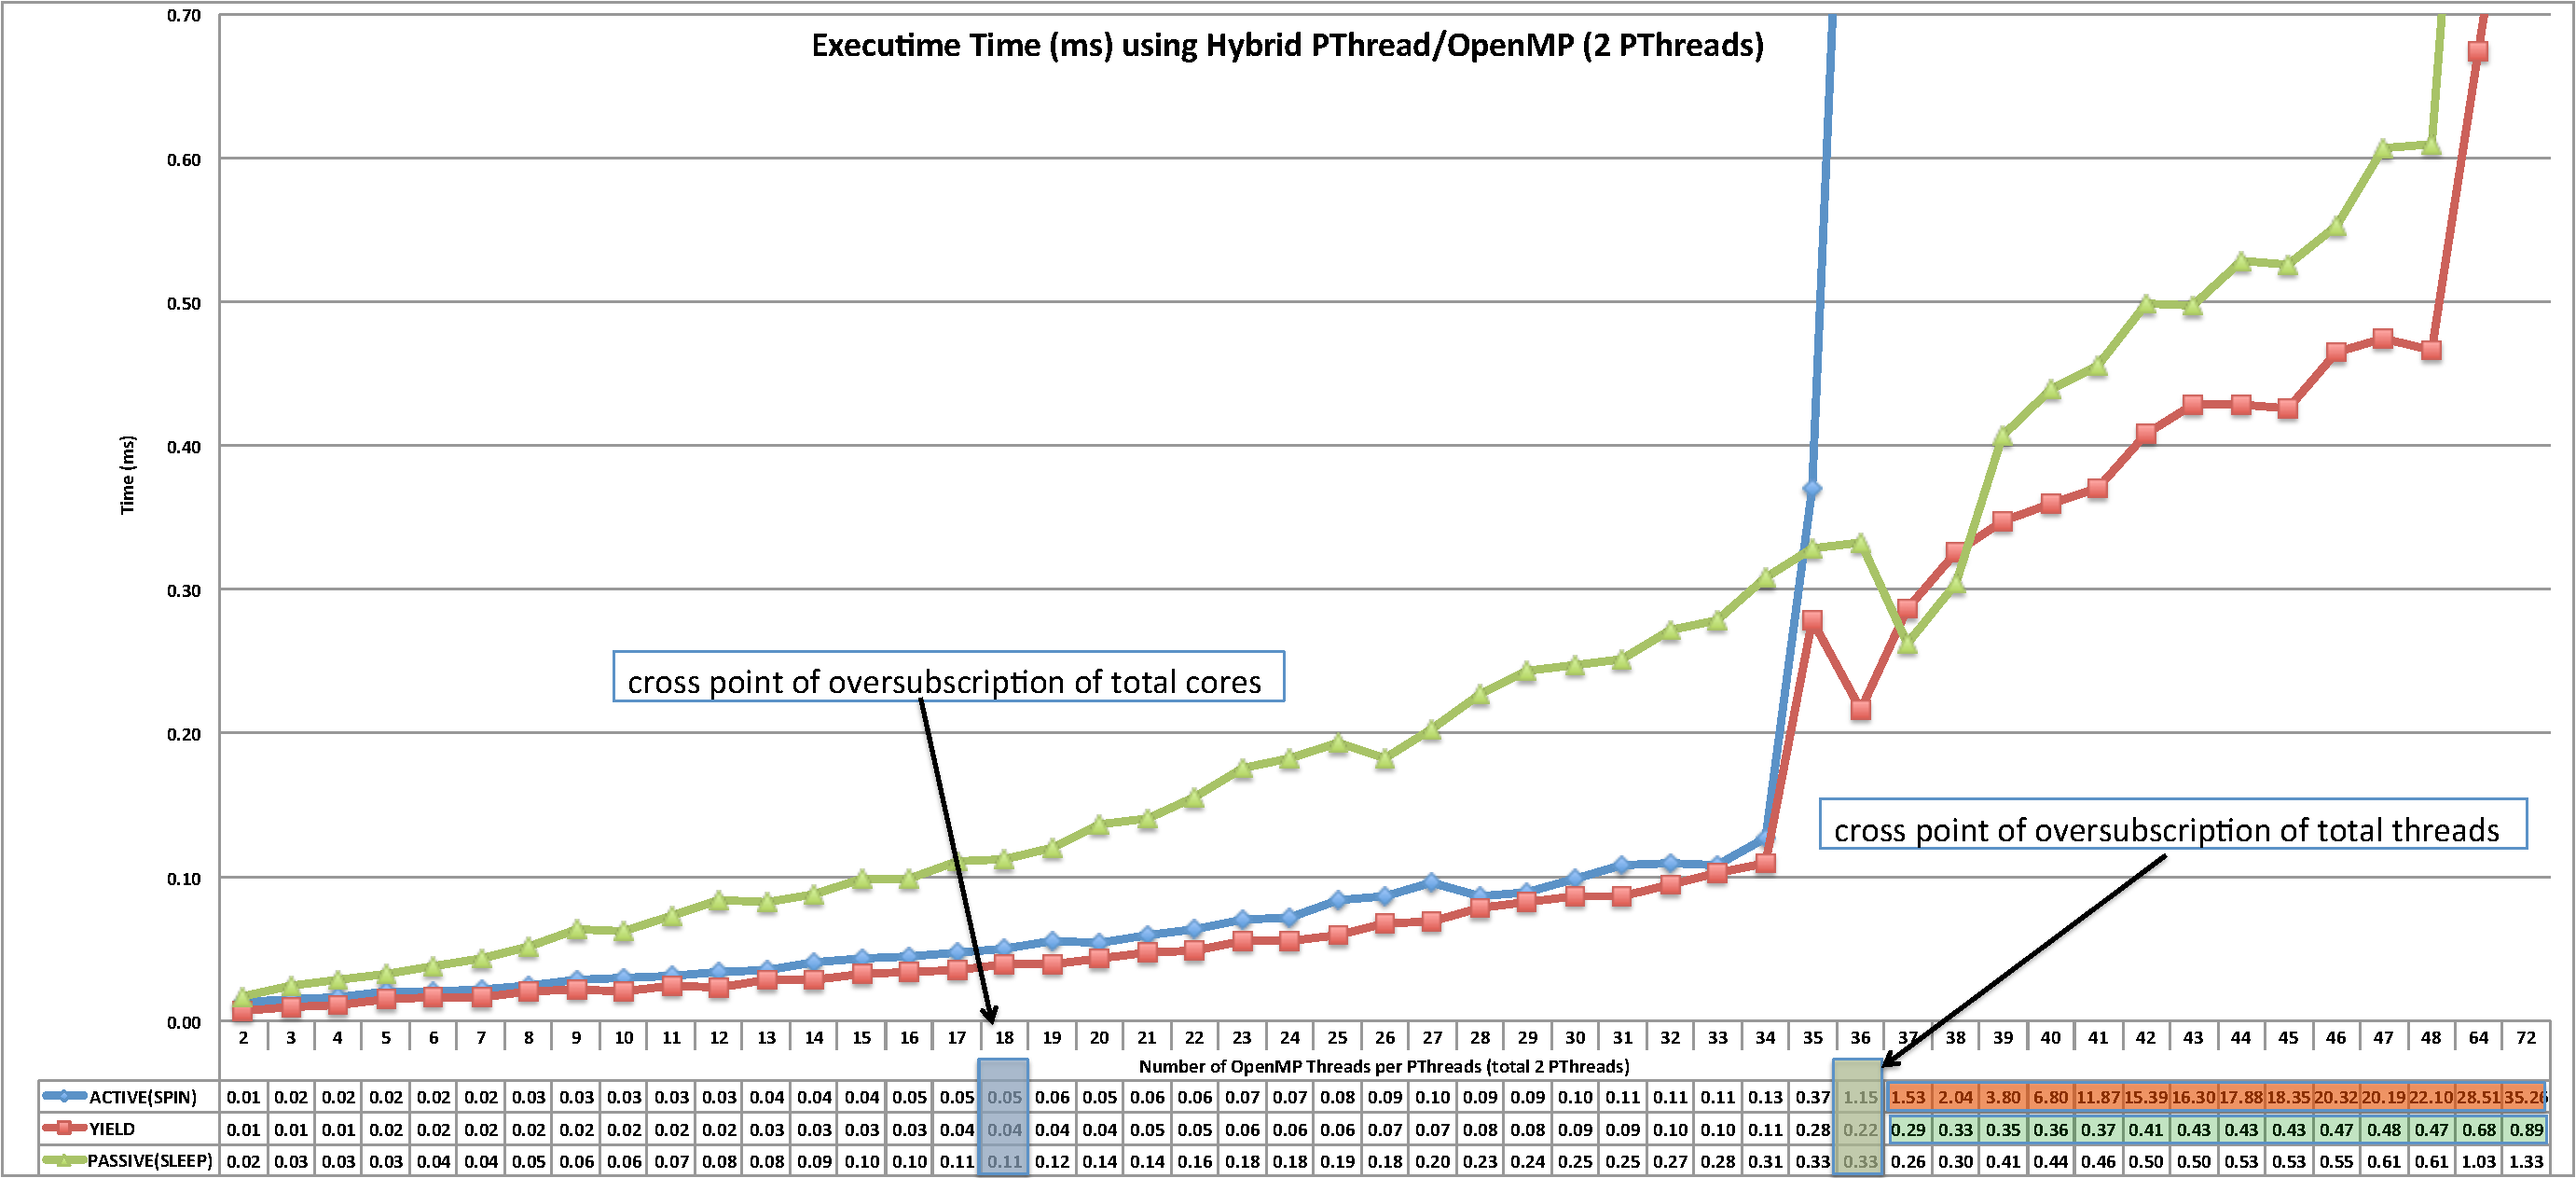
\includegraphics[width=0.99\textwidth] {images/2PThread_performance}
    \caption{Performance (ms) for hybrid PThreads/OpenMP execution: 2 PThreads and the system has total 36 cores for 72 threads.}
    \label{fig:2PThread_performance}
\end{figure}

\begin{figure}[h]
    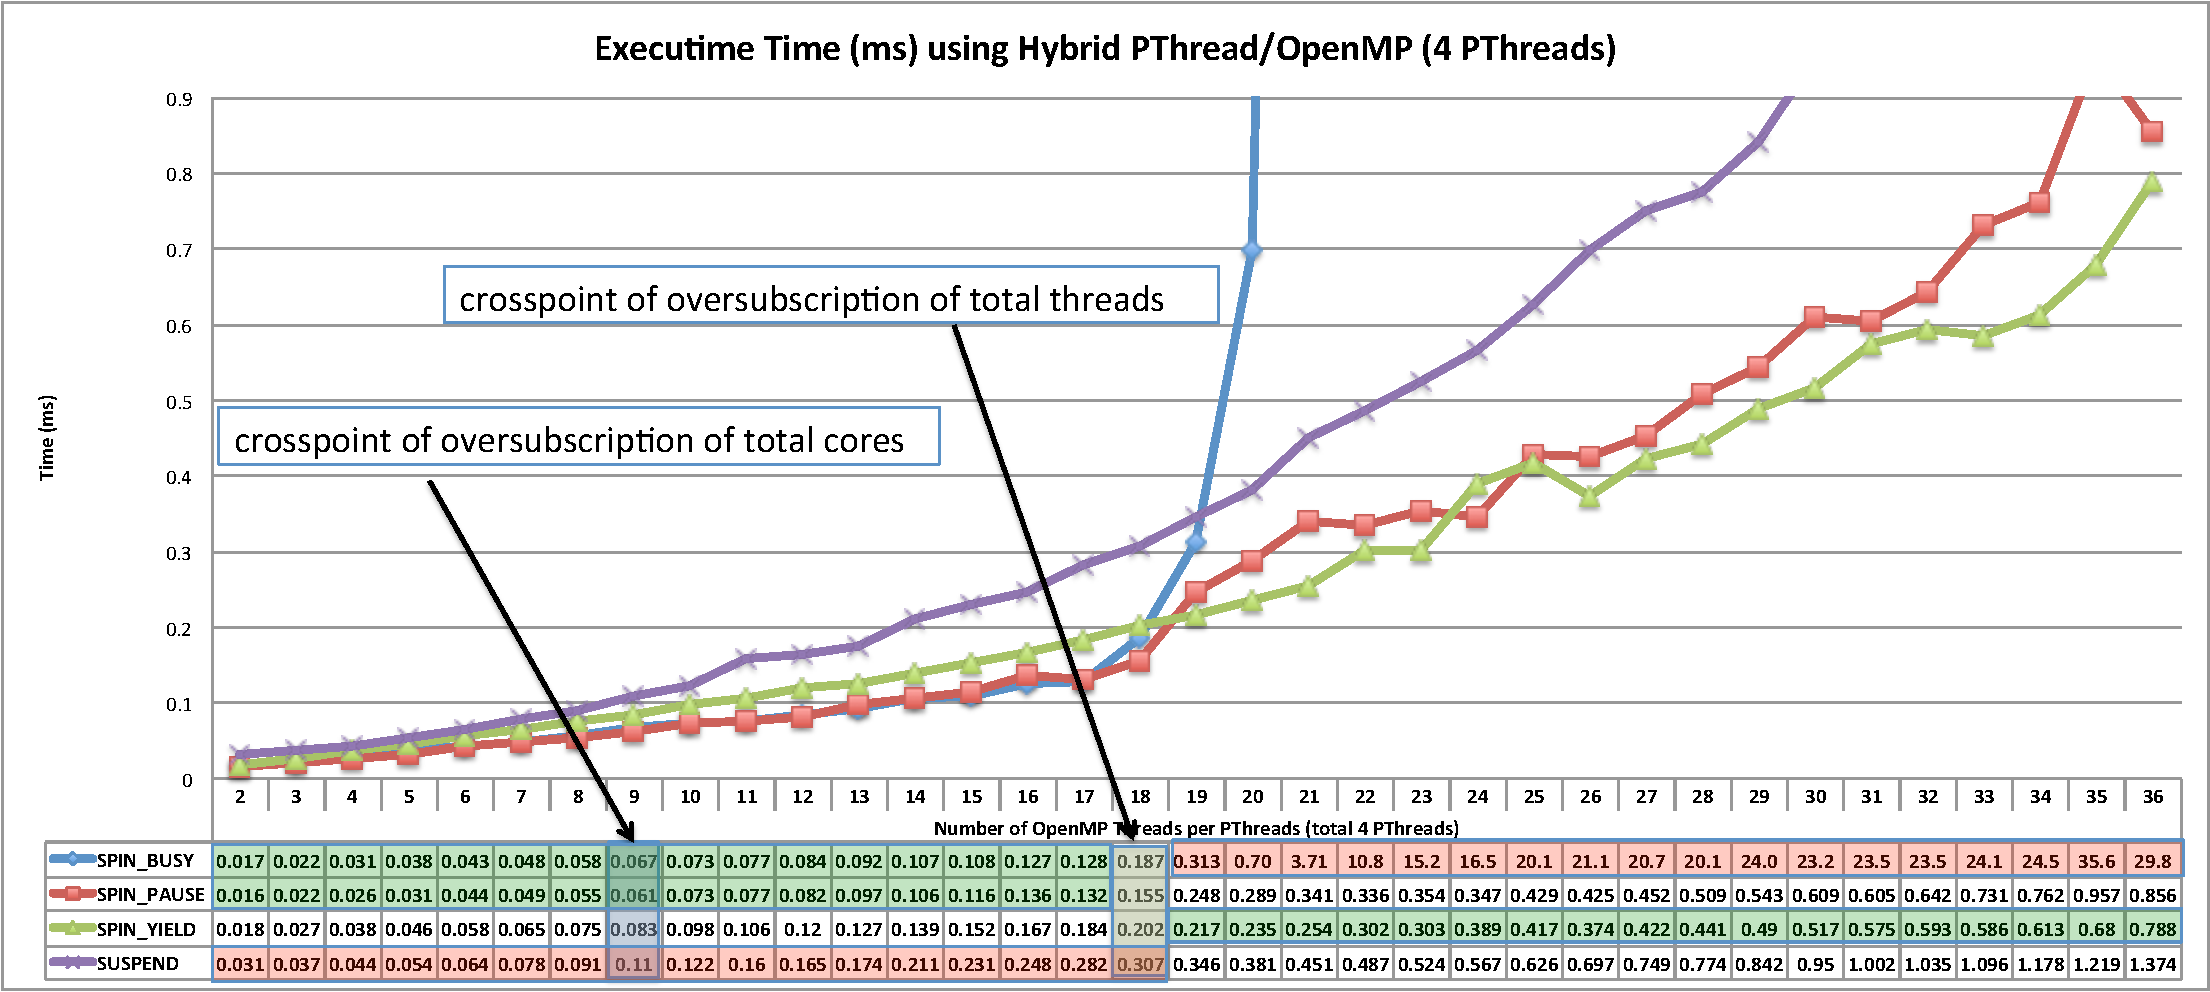
\includegraphics[width=0.99\textwidth] {images/4PThread_performance}
    \caption{Performance (ms) for hybrid PThreads/OpenMP execution: 4 PThreads and the system has total 36 cores for 72 threads.}
    \label{fig:4PThread_performance}
\end{figure}

\begin{figure}[h]
    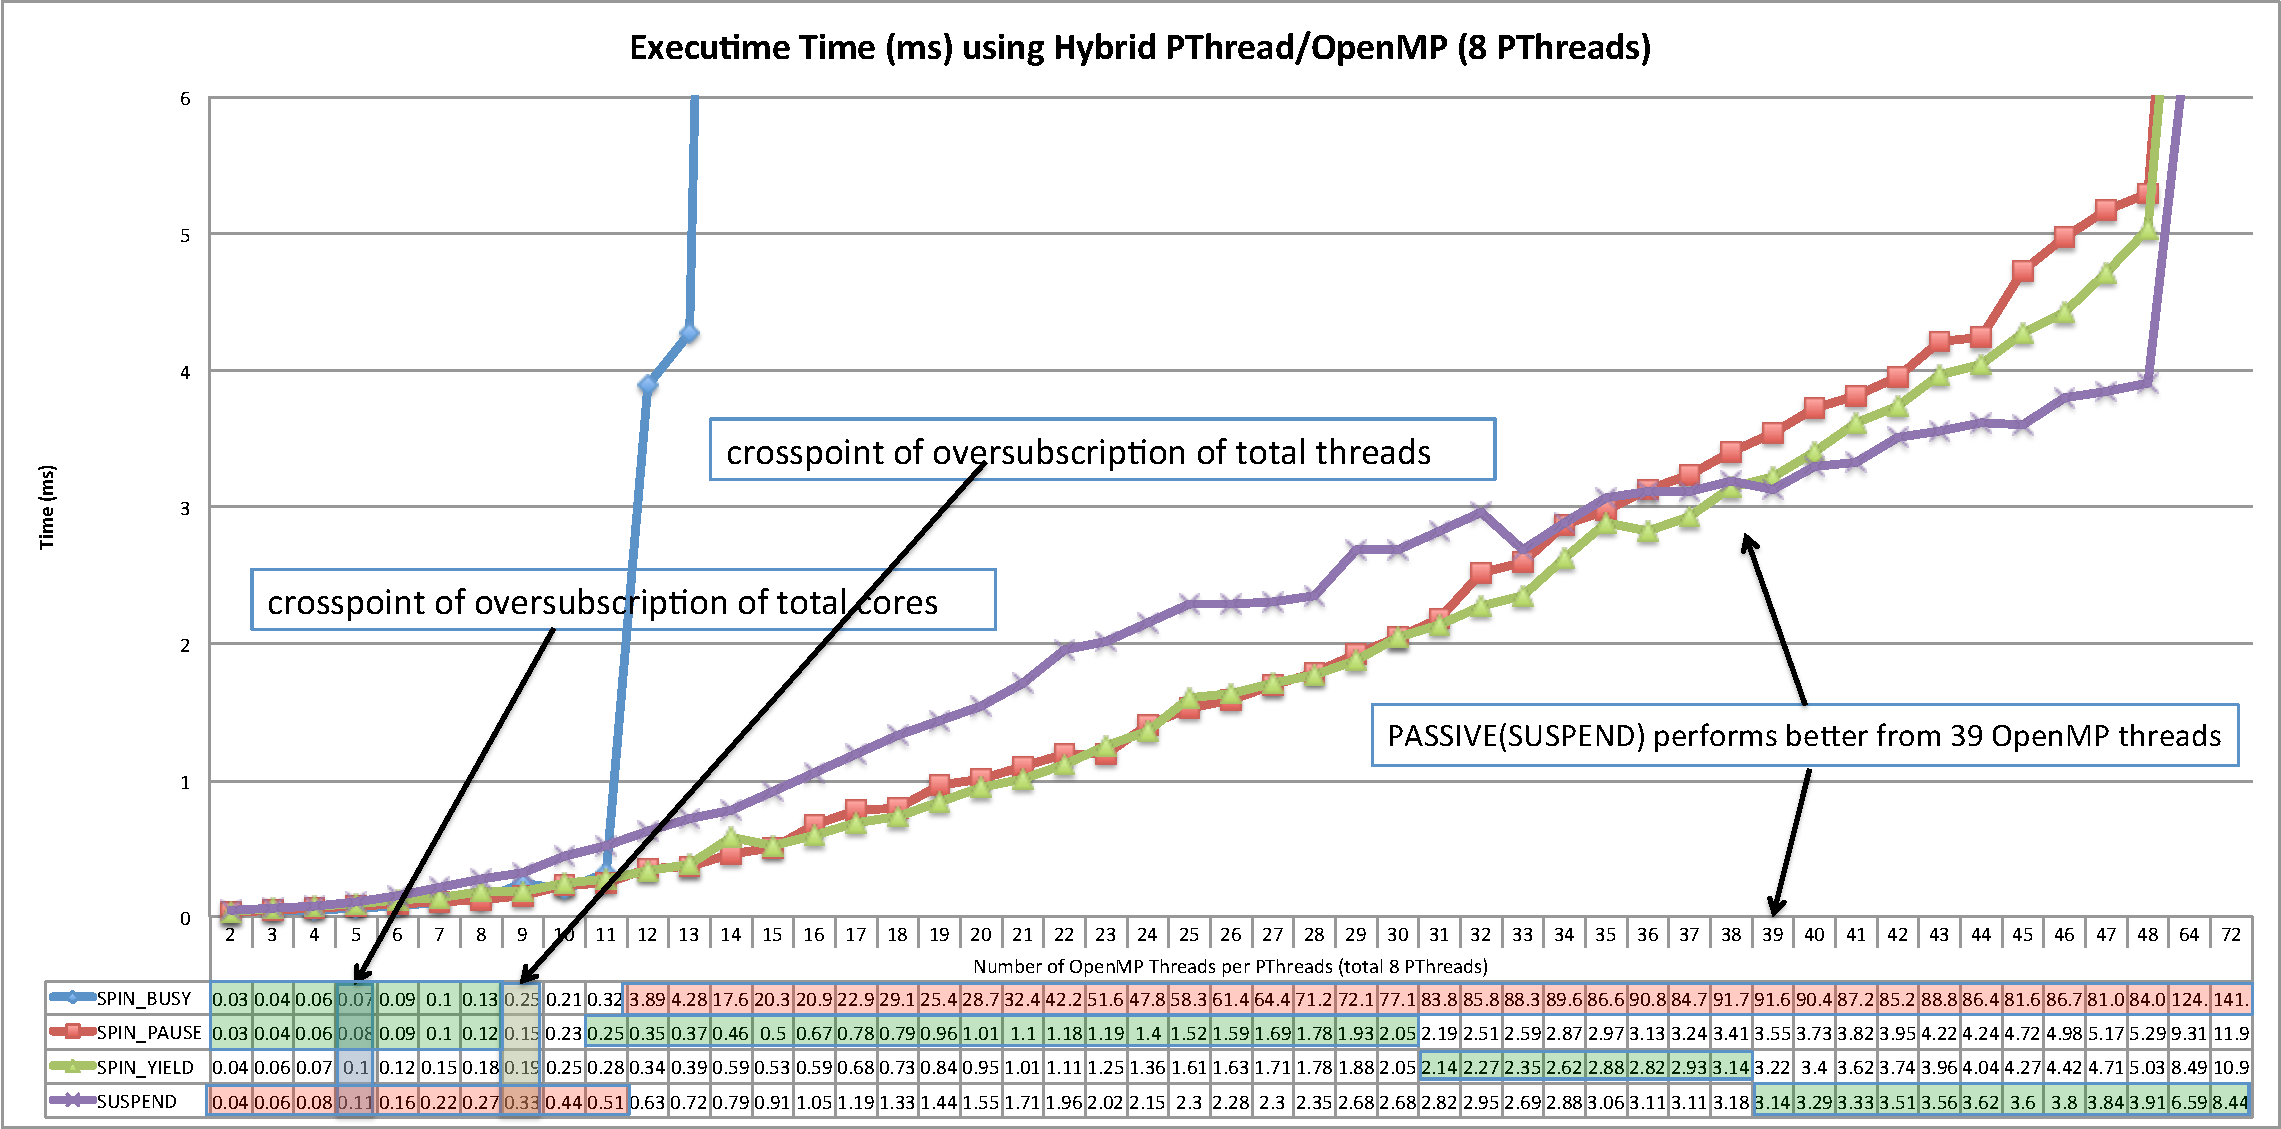
\includegraphics[width=0.99\textwidth] {images/8PThread_performance}
    \caption{Performance (ms) for hybrid PThreads/OpenMP execution: 8 PThreads and the system has total 36 cores for 72 threads.}
    \label{fig:8PThread_performance}
\end{figure}

The evaluation results using 2, 4, and 8 PThreads, each of which creates {\sf parallel} region ranging 
from 2 to 72 threads, are shown in Figure~\ref{fig:2PThread_performance},~\ref{fig:4PThread_performance} 
and~\ref{fig:8PThread_performance}. We marked the two crosspoints for each configuration in the figure and the 
policy that delivers the best performance is highilighted in green color and the worest performance in red color.
The results clearly show the effectiveness of using wait policies. For all the three configurations, 
before the crosspoint \#2 from which oversubscription just starts to occur, 
the two {\sf ACTIVE} wait polices, ({\sf SPIN\_BUSY} and {\sf SPIN\_PAUSE}, deliver the best performance and 
the {\sf PASSIVE SUSPEND} delivers the worest (max 2x time slower). 
The {\sf PASSIVE SPIN\_YIELD} delivers slightly worse performance than the two {\sf ACTIVE} policies, but still much better than the 
{\sf PASSIVE SUSPEND} policy. 
It can be explained that minumum overhead from OS kernel scheduling and context switch is incurred since 
the program does not oversubscribe the hardware threads. 
All the results also show that there are not much changes of the performance by those policies when crossing the crosspoint \#1. 
%It is very interesting that the YIELD policy performs
%consistently better than SPIN policy, indicating that even there is no oversubscription, SPIN waiting is not 
%the best option for optimal interoperability and performance.

After passing the crosspoint \#2, the results in the three figures also clearly show the dramatic increase 
of the execution time (5x to 10x) when using the {\sf ACTIVE SPIN\_BUSY} policy. 
This policy does not help address oversubscription because of the large amount of overhead from OS kernel thread scheduling and context switch 
incurred when the threads are competing for hardware cores. The mild increase
of the execution time when using either {\sf ACTIVE SPIN\_PAUSE} or {\sf PASSIVE SPIN\_YIELD} 
policy clearly shows effect of the two policies to address
the oversubscription issue. The {\sf PASSIVE SPIN\_YIELD} also performs better than {\sf ACTIVE SPIN\_PAUSE} policy. 
We also observed that the two policies consistently outperform the {\sf PASSIVE SUSPEND}
policy (20\% to 40\%) for the configuration using 2 and 4 PThreads. The 8-PThread configuration shows that the 
 {\sf PASSIVE SUSPEND} policy outperforms the other policies from 38 OpenMP threads/PThread onwards for as much as 35\%. 
 This indicates that for a program that heaviliy oversubscribes hardware resources, the {\sf PASSIVE SUSPEND} 
 policy is a better option among the four.

\subsection{Performance With Regards to the Oversubscription Ratio}
To future study the effects of the four wait policies and the approach for selecting an optimal policy for different
configurations, we introduce the term oversubscription ratio as the ratio of total number of
threads requested by a program to the total number of hardware threads. If the ratio is less than or equal to 1,
there is no oversubscription (assuming the program uses all the hardware threads of the system). 
In figure~\ref{fig:ovratio}, we consolidate the results from the previous three figures and plot with regards to 
the oversubscription ratio. The left figure shows that when the ratio is less than 1.0 (no oversubscription), 
the {\sf ACTIVE} {\sf SPIN\_BUSY} and {\sf SPIN\_PAUSE} 
deliver similar and better performance over other policies. 
When the ratio is between 1.0 to 4.0 (mild oversubscription), the {\sf ACTIVE SPIN\_PAUSE} and {\sf PASSIVE SPIN\_YIELD} policies 
perform similar and consistently better than others, but being gradualy caught up by the {\sf PASSIVE SUSPEND} policy as the ratio increases. 
The {\sf ACTIVE SPIN\_BUSY} performs very poorly right after the ratio passes 1.0. 
When the ratio is above 4.0 (heavy oversubscription), the {\sf PASSIVE SUSPEND} policy performs the best. 
\begin{figure}[h]
    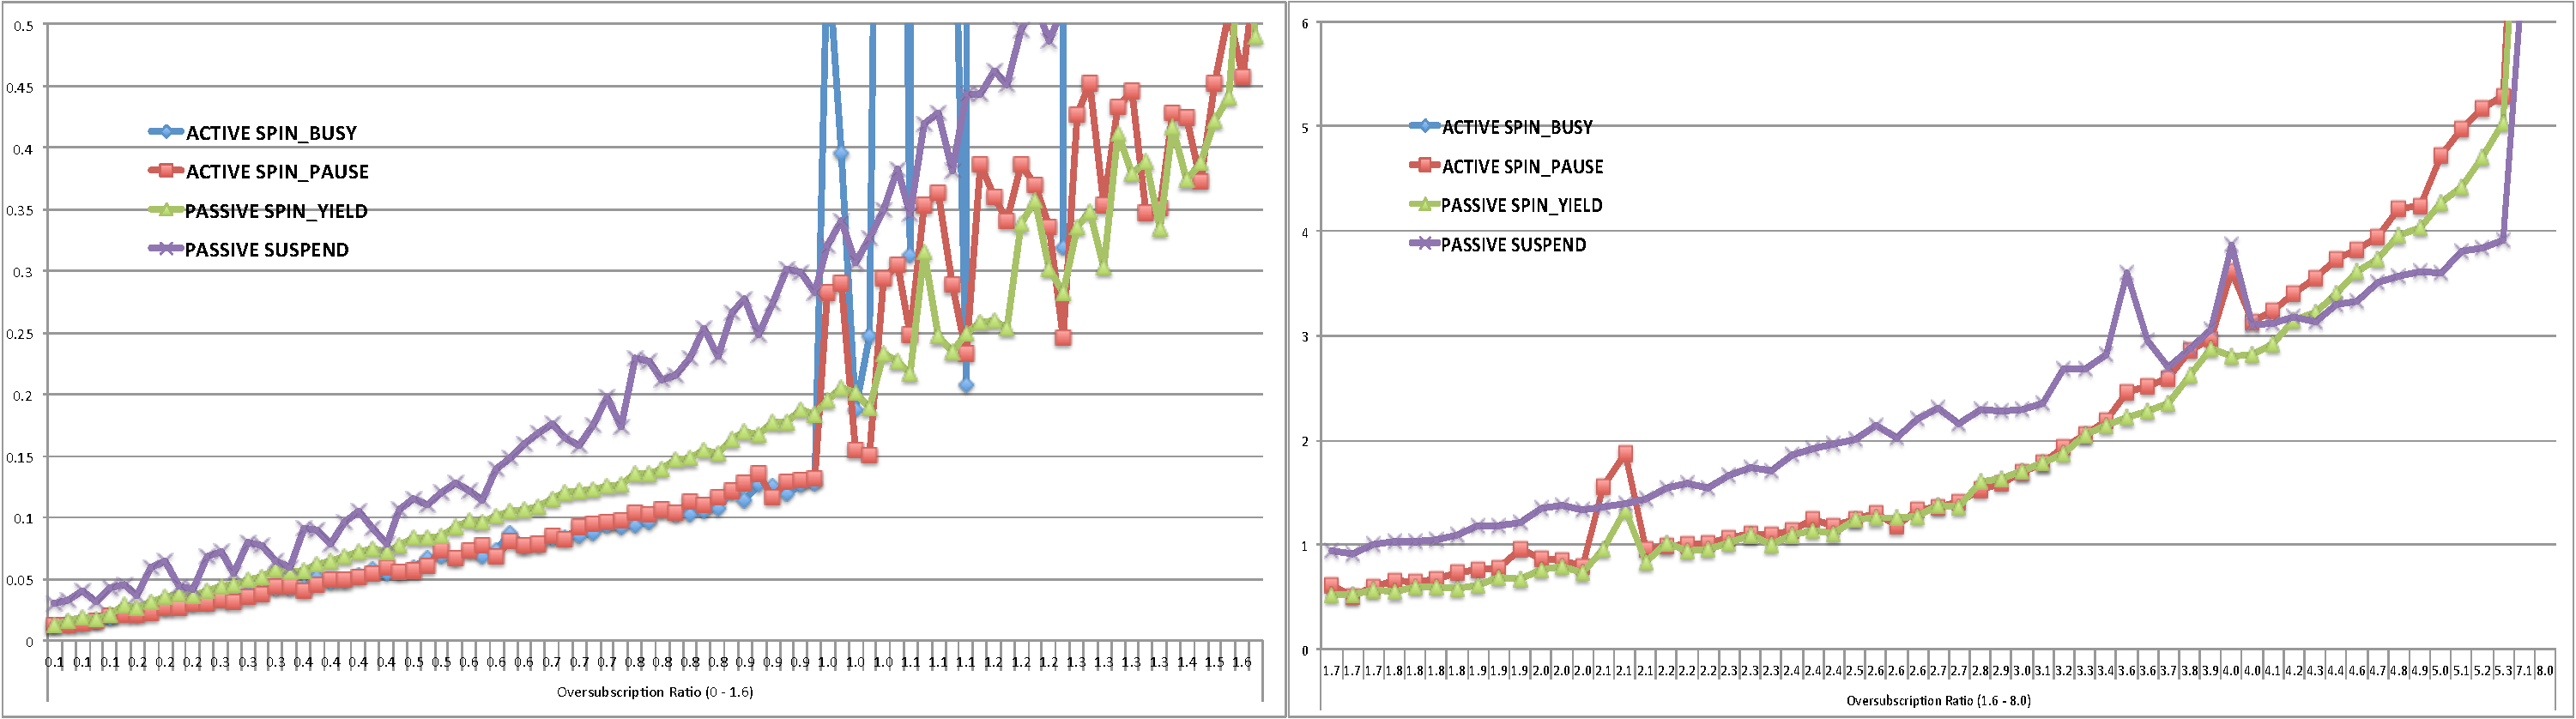
\includegraphics[width=0.99\textwidth] {images/ovratio}
    \caption{Performance (ms) of using different wait policy with regards to the oversubscription ratio}
    \label{fig:ovratio}
\end{figure}

As a summary, the evaluation demonstrates the effectiveness of the wait policy for combating the performance 
impacts of oversubscription. Heuristics for selecting the right policy 
could be drawn from this single but representative experiment as follows:
The {\sf ACTIVE SPIN\_BUSY} or {SPIN\_PAUSE} policy should be used when there is no oversubscription. 
For mild oversubscription (ratio less than 4), both {\sf ACTIVE SPIN\_PAUSE} and {\sf PASSIVE SPIN\_YIELD} are good options. 
For heavily oversubscribed system, the {\sf PASSIVE SUSPEND} policy should be 
considered to best coordinate resources between parallel runtime. 

%because the OpemMP just creates that once. Then, it puts them in a global thread pool to be used next time needed. However, the time cost represented by the quiesce term refers to the time required to shutdown the whole runtime library. In other words, after each parallel region we remove all threads in the global thread pool. Finally, the startup{\_}quiesce term implies the time required to initialize the parallel region and the time taken to shutdown the runtime library. 

% FUSED FIGURE

% ORIGINAL FIGURE
\begin{comment}
\begin{figure}[ht]
    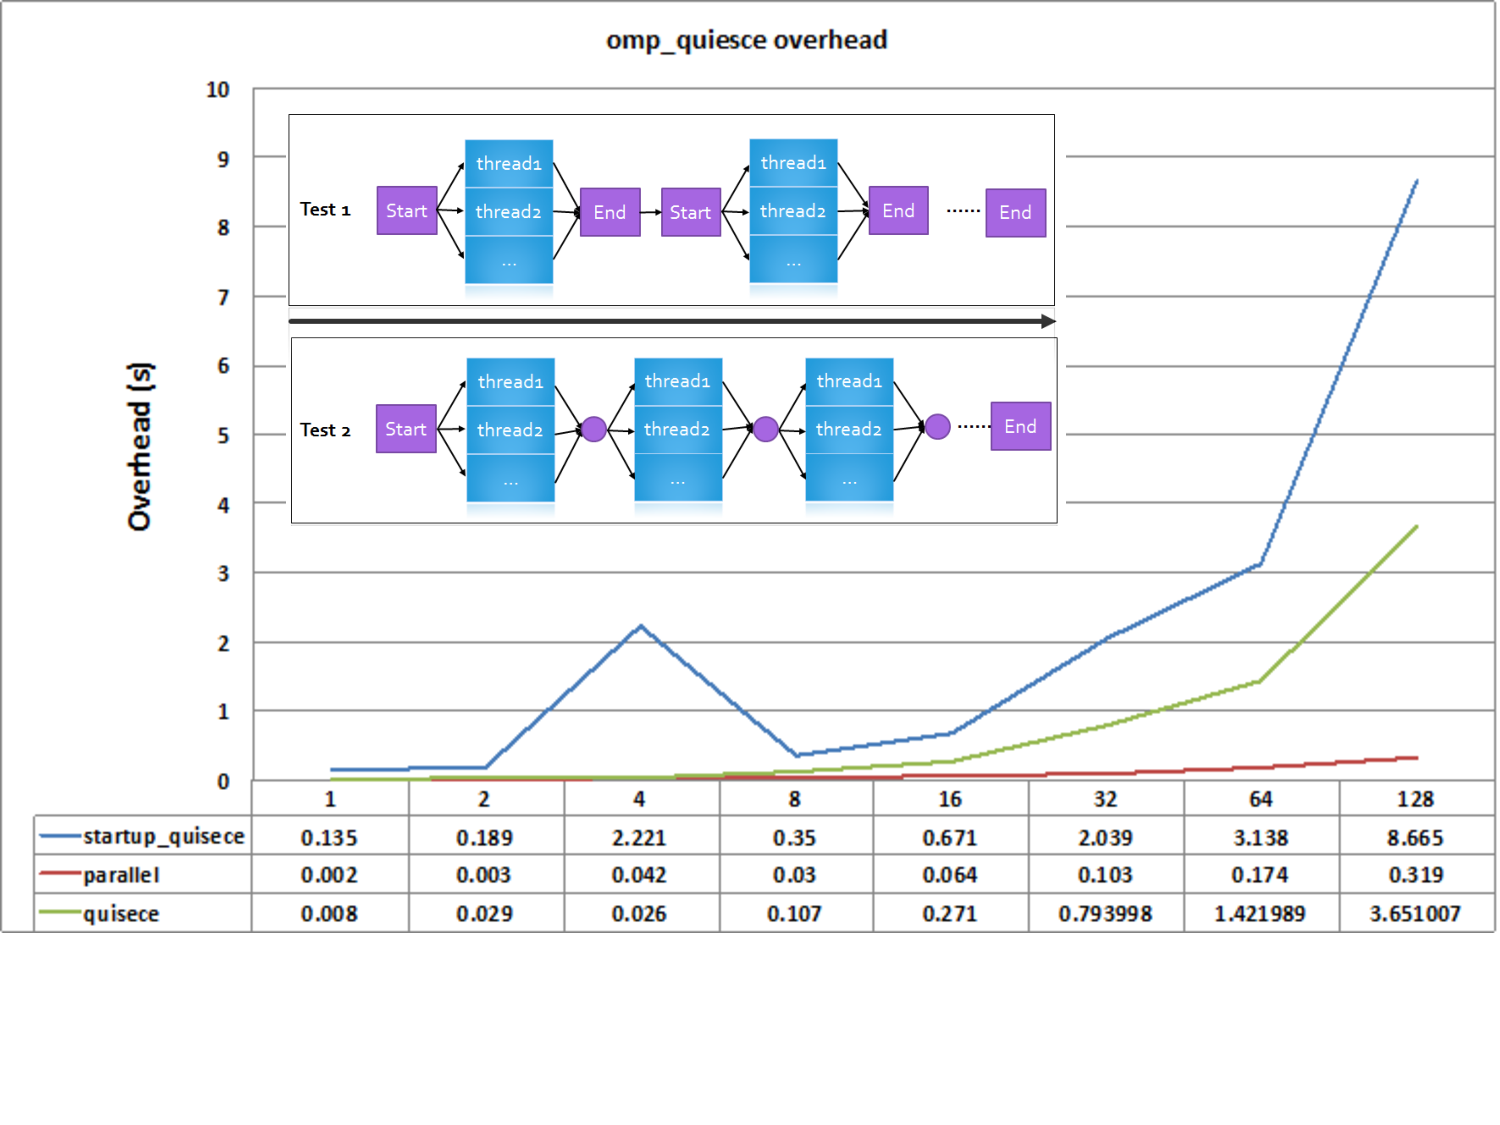
\includegraphics[width=0.9\textwidth] {images/omp_quiesce_fusion}
    \caption{{\sf omp\_quiesce} evaluation.}
    \label{omp:quiesce_evaluation}
\end{figure}
%\vspace{-0.6cm}
\begin{figure}[ht]
\subfigure[Test Design]{
		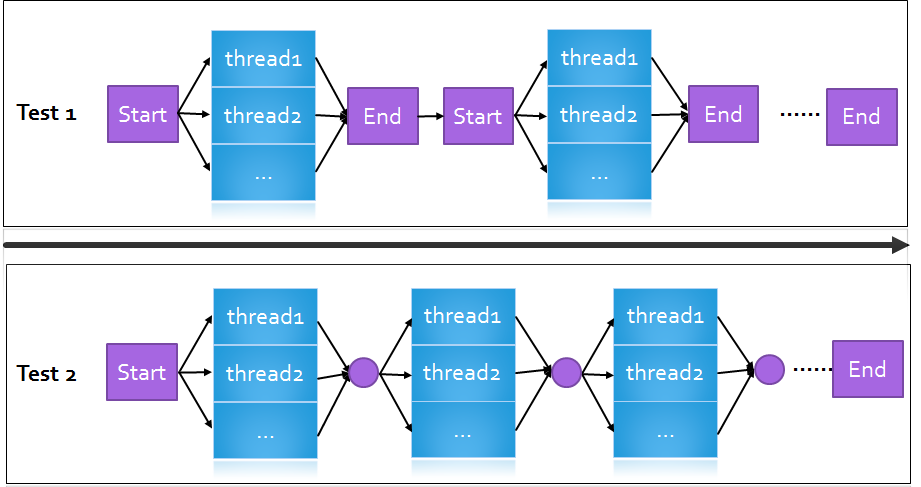
\includegraphics[width=0.6\textwidth] {images/quiesce_evaluation}
		\label{omp:quiesce_evaluation}
}
\subfigure[Evaluation Results]{
		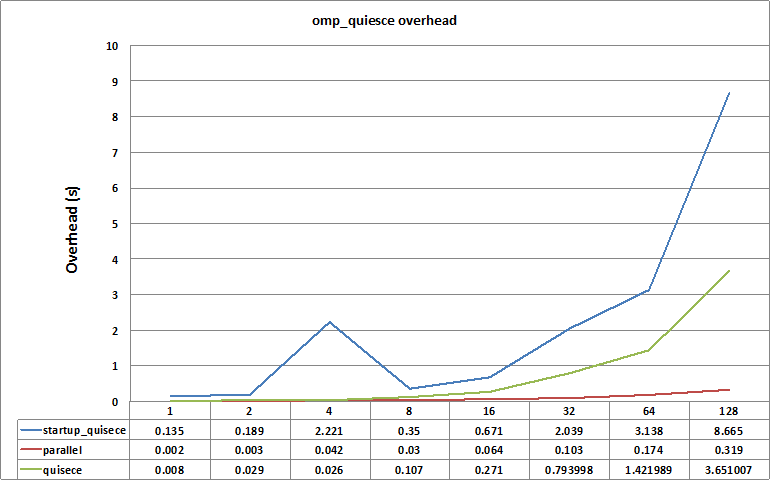
\includegraphics[width=0.6\textwidth] {images/quiesce_results}
		\label{omp:quiesce_results}
}
\caption[]{{\sf omp\_quiesce} Evaluation}
\label{fig:quiesce}
\end{figure}
%\vspace{-0.4cm}
\end{comment}


\REM{

\begin{enumerate}
	\item void omp{\_}quiesce()
	\item void omp{\_}set{\_}wait{\_}policy(PASSIVE \textbar ACTIVE)
	
	We need to create two processes since each process will only maintain and share one thread pool. For those two process, each task is execute using 1s, and we need to create enough threads to make full use of the calculation power of one CPU. We tested it in three cases: passive, active, and quiesce/restart the runtime environment. Figure~\ref{omp:wait_policy_evaluation} shows the design of the evaluation.
	
	\begin{figure}
		\centering
		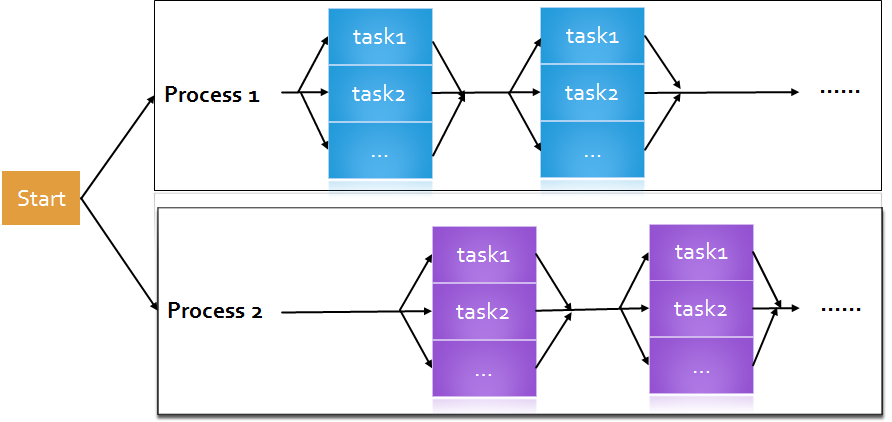
\includegraphics[width=0.7\textwidth] {images/wait_policy_evaluation}
		\caption{waiting policy evaluation}
		\label{omp:wait_policy_evaluation}
	\end{figure}
	
	As Figure~\ref{omp:wait_policy_results} below shows, there is no a big difference between the two behaviors. The reason is that the OpenMP uses only one global thread pool for all OpenMP threads created by multiple PThreads. So, the small difference comes from the time required to awake a sleeping thread. By doing this experiment, we have understand more about the way that OpenMP deals with the thread pool. 
	
	\begin{figure}
		\centering
		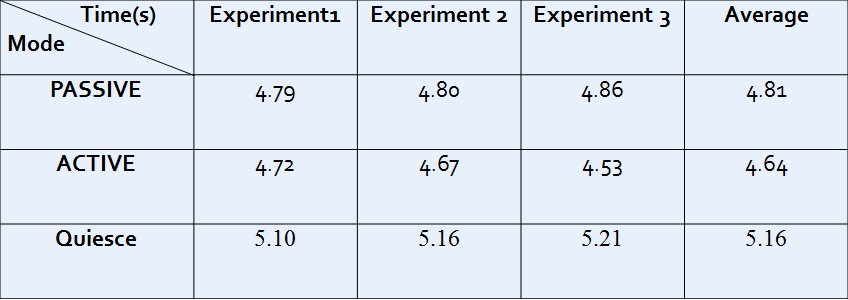
\includegraphics[width=0.7\textwidth] {images/wait_policy_results}
		\caption{Waiting Policy Results}
		\label{omp:wait_policy_results}
	\end{figure}
	
	
	\item int omp{\_}thread{\_}create()
	
	We compared this function with creating pthread to execute a list of tasks. So, for this function we have tested it in two different ways. Figure~\ref{omp:create_evaluation} shows the design of the evaluation. For the first way, we put different number of tasks in one parallel region, so that every “omp{\_}thread{\_}create()” or “pthread{\_}create()” function will be run in parallel. On the other hand, we use different iterations to execute the “omp{\_}thread{\_}create()” or “pthread{\_}create()” functions in sequence, and compare the running time. 
	
	\begin{figure}
		\centering
		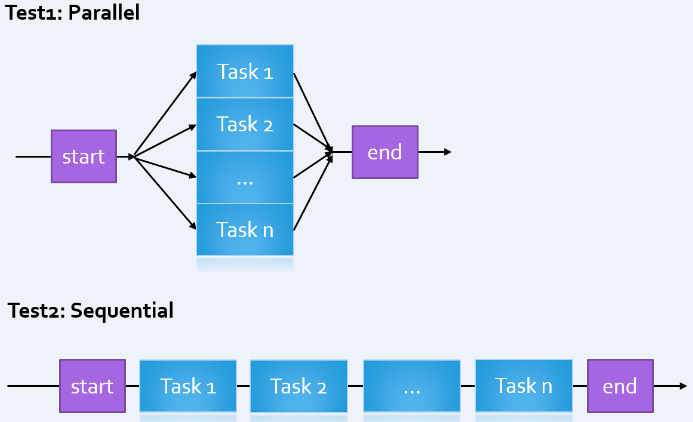
\includegraphics[width=0.7\textwidth] {images/create_evaluation}
		\caption{creating thread evaluation}
		\label{omp:create_evaluation}
	\end{figure}
	
	Figure~\ref{omp:create_results_parallel2} and Figure~\ref{omp:create_results_parallel} show the result of the first approach (execute in parallel). It clearly shows that there is almost no differences between them. This is might be because that we are doing it inside the parallel region.However, Figure~\ref{omp:create_results_sequence2} and Figure~\ref{omp:create_results_sequence} show the result of the second approach (execute in sequence). They show that omp{\_}thread{\_}create() gives a better performance that pthread{\_}create( ). So, it would be a good feature if the user can do this instead of creating another pthread.

% I do not think we need these.  The performance should be relatively obvious
% and in any case should not matter.  The purpose is to create an OS thread
% that the OpenMP runtime is aware of, and otherwise it should be the thinnest
% possible wrapper about the native OS thread library.
% Because of this, I do not see how omp_thread_create can be faster than
% pthread_create.
%                       - Jeff
\begin{comment}
	\begin{figure}
		\centering
		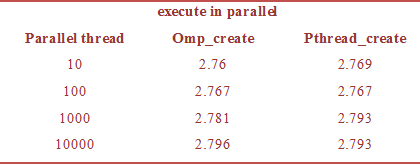
\includegraphics[width=0.7\textwidth] {images/create_results_parallel2}
		\caption{Results of omp\_thread\_create in parallel}
		\label{omp:create_results_parallel2}
	\end{figure}
	\begin{figure}
		\centering
		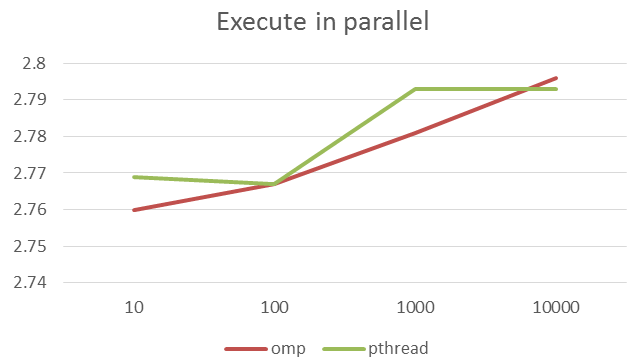
\includegraphics[width=0.7\textwidth] {images/create_results_parallel}
		\caption{Results of omp\_thread\_create in parallel}
		\label{omp:create_results_parallel}
	\end{figure}
	\begin{figure}
		\centering
		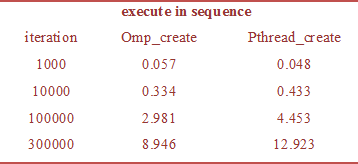
\includegraphics[width=0.7\textwidth] {images/create_results_sequence2}
		\caption{Results of omp\_thread\_create in sequence}
		\label{omp:create_results_sequence2}
	\end{figure}
	\begin{figure}
		\centering
		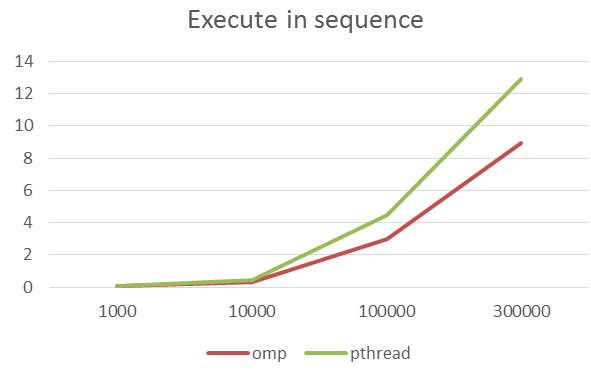
\includegraphics[width=0.7\textwidth] {images/create_results_sequence}
		\caption{Results of omp\_thread\_create in sequence}
		\label{omp:create_results_sequence}
	\end{figure}
\end{comment}

\end{enumerate}

}


 
%\section{Hierarchical Place Trees (HPT) Model} 
%\label{sec:model}
%\input{modeling}

%\section{Programming Interface and Implementation}
%\label{sec:interface}
%\input{interface}

%\vspace{-0.8cm}
%\section{Preliminary Experimental Results}
%\label{sec:eva}
%\input{eva}

\section{Related Work}
\label{sec:related}
Some previous studies have studied the interoperability and composibility of parallel programming models and libraries. 
Tian et al.~\cite{tian2003compiler} explored interoperability between OpenMP threads and system threads (e.g. pthreads and WinThreads) in Intel OpenMP compilers.
For ease of use for programmers, they decided not to share thread identifiers between system threads and their OpenMP parent
and not to share threadprivate variables among system threads.
Also, a forked system thread calling \lstinline{omp_in_parallel()} would return false, even if it is created by an OpenMP thread. 

Callisto~\cite{Callisto:Harris:2014:CCP:2592798.2592807} and
Lithe~\cite{Lithe:Pan:2009:LEE:1855591.1855602} 
address the interoperability challenge 
through the design of a low-level software layer for common 
resource management underneath multiple parallel runtime systems, such as OpenMP and TBB. % of programming models. 
%They however do not address the algorithm conflicts of different runtime systems. 
The MPC (Multi-Processor Computing) framework~\cite{perache2008mpc} is a unified parallel runtime designed for clusters of large NUMA nodes. 
Through process virtualization and thread-based MPI implementation, MPC enables efficient mixing of MPI, OpenMP, and Pthreads. 
In order to compose multiple simultaneously executing parallel applications, Hugo et al.~\cite{hugo2014composing} extends the starPU runtime system to allow confined execution environments (called scheduling contexts) which can be used to partition computing resources. 
A hypervisor is used to automatically expand or shrink contexts based on runtime resource utilization feedback. 

The MPI endpoints~\cite{Dinan:mpiendpoint_eurompi13}
proposal to the MPI standard relaxes the one-to-one relationship between processes and ranks.
It allows registering a thread in an MPI
process as a MPI communicator rank that is able to independently paraticipate
in message passing operations. There are also efforts of integrating MPI calls as
tasks in a intra-node workstealing runtime~\cite{hcmpi:ipdps13}.

For enable interoperability among distributed HPC programming models, Epperly et al.~\cite{epperly2011composite} proposed a mixed-language environment supporting arbitrary combination of software written in PGAS languages (Co-Array Fortran, UPC, and Titanium) and HPCS languages (Chapel, X10, and Fortress). 
They designed the Scientfic Interface Definition Laguage (SIDL) and Babel Intermediate Object Representation (IOR) as a language-independent object-oriented programming model and type system
to allow software components to share complicated data structures across various languages. 

%\FloatBarrier
\section{Conclusions and Future Work}
\label{sec:conclusion}
In this paper, we have explored use cases for OpenMP to interact with itself and other programming models
in order to expose OpenMP's iteroperability challenges. 
We have proposed a set of extensions to OpenMP to support multiple levels of interoperability functionalities. 
%seen that there are many features can be added to the current 
Ongoing implementation is being done using two OpenMP runtime libraries, with initial results for 
interoperability functions for setting wait policies, shutting down runtime, and creating user threads, etc. 
\begin{comment}
One feature is 
that allowing the user to create a new OpenMP thread and assign a task to it instead 
of creating new user thread. We have implement a function to allow users to get one 
thread from the existing thread pool is any threads are available, and assign one task 
to this thread, this helps to take advantage of the OpenMP thread pool and won’t need 
to create a new thread to work on it, which helps to save the memory usage and speed up the runtime.

We have studied the waiting policy of the OpenMP and how the current OpenMP Runtime System deals with the thread pool. Considering there are two waiting policies, one called throughput (passive), which is designed to make the program aware of its environment (that is, the system load) and to adjust its resource usage to produce efficient execution in a dynamic environment. While the other one called turnaround (active), which is designed to keep active all of the processors involved in the parallel computation in order to minimize the execution time of a single job. We cannot simply say which one is better than the other, it depends one the executing environment. When setting the wait policy to be passive, after a certain period of time has elapsed, the useless thread will stop waiting and sleep. Thus active mode may be better for high-density of OpenMP tasks. While, a passive mode with a small blocktime value may offer better overall performance if your application contains non-OpenMP threaded code that executes between parallel regions. 

In addition, we have implemented a new function to shutdown the whole runtime library when exiting the parallel region. Since all threads are maintained in the same thread pool, quiesce will reap every threads to free the memory, which sometimes help to clear the runtime environment when the task density is lower and we don’t need to wake up most of the thread in the thread pool. However, when entering new parallel regions, we need to make sure that we register the current working thread as our root thread, so that new runtime environment can be built on it. It cost time to restart another parallel region, thus works slower when lots of tasks in the task queue.
\end{comment}

For future work, we will continue adding more proposed interoperability functionalities into the existing runtime systems. We will conduct in-depth evaluation using representative benchmarks to demonstrate the benefits of OpenMP runtime systems with better interoperability. 
%By doing this, we could have a better OpenMP runtime library that optimizes the resources utilization.

%\vspace{-0.1in}
\section*{Acknowledgments}
%The solutions are based on the various discussions from 
We thank members from the OpenMP Interoperability language subcommittee and the language 
committee in general for providing insightful comments of the design. 
%We particularly appreciate Alexandre Eichenberger from IBM for . 
We are also grateful to Terry Wilmarth and Brian Bliss from Intel for providing information for our 
implementation. 
This material is based upon work supported by the National
Science Foundation under Grant No. SHF-1409946 and SHF-1551182. 
This work performed under the auspices of the U.S. Department of Energy by Lawrence Livermore National Laboratory under Contract DE-AC52-07NA27344.
% to stay within page limit, remove for now
%\scriptsize{
%    ~\\
%    \noindent\othertm{}Other names and brands may be claimed as property of others.
%
%    \noindent
%    Intel and Xeon are trademarks of Intel Corporation in the U.S. and/or other countries.
%    Software and workloads used in performance tests may have been optimized
%    for performance only on Intel microprocessors.  Performance tests, such as
%    SYSmark and MobileMark, are measured using specific computer systems,
%    components, software, operations and functions.  Any change to any of those
%    factors may cause the results to vary.  You should consult other information
%    and performance tests to assist you in fully evaluating your contemplated
%    purchases, including the performance of that product when combined with
%    other products.  For more information go to \url{http://www.intel.com/performance}.
%}

\small{
\bibliographystyle{plain}
%IEEEtran}
%\nocite{*}
\bibliography{IEEEabrv,interop}
}
\end{document}
